\documentclass[12pt,oneside,a4paper,reqno]{book}
\usepackage{amsmath,amsxtra,amssymb,latexsym, amscd,amsthm,}
\usepackage{amsfonts}
\usepackage[portrait, top=3.5 cm, bottom=3cm, left=3.5cm, right=2.5cm] {geometry}

\usepackage[utf8]{vietnam}
\usepackage{varioref}

\usepackage{fancyhdr}
\usepackage{longtable}
\usepackage{graphicx}
\usepackage{fancybox}
\usepackage{color, graphicx}
\usepackage{verbatim}
\usepackage{tabularx}
\usepackage{wrapfig}
\usepackage{setspace}
\setlength{\baselineskip}{16truept}
\renewcommand{\baselinestretch}{1.45}
%\renewcommand{\baselineskip{1.5}}
%\usepackage[colorlinks,citecolor=black,filecolor=black,linkcolor=black,urlcolor=black]{hyperref}

\newtheorem{dn}{Định nghĩa}[chapter]
\newcommand{\bdn}{\begin{dn}\rm}
\newcommand{\edn}{\end{dn}}

\newtheorem{nx}{Nhận xét}[chapter]
\newcommand{\bnx}{\begin{nx}\rm}
\newcommand{\enx}{\end{nx}}

\renewcommand{\tabularxcolumn}{m}


\newtheorem{md}{Mệnh đề}[chapter]
\newcommand{\bmd}{\begin{md}}
\newcommand{\emd}{\end{md}}

\newtheorem{hq}{Hệ quả}[chapter]
\newcommand{\bhq}{\begin{hq}}
\newcommand{\ehq}{\end{hq}}

\newtheorem{bd}{Bổ đề}[chapter]
\newcommand{\bbd}{\begin{bd}}
\newcommand{\ebd}{\end{bd}}

\newtheorem{tc}{Tính chất}[section]
\newcommand{\btc}{\begin{tc}}
\newcommand{\etc}{\end{tc}}

\newtheorem{vd}{Ví dụ}[section]
\newcommand{\bvd}{\begin{vd}\rm}
\newcommand{\evd}{\end{vd}}

\newtheorem{cm}{Chứng minh}[section]
\newcommand{\bcm}{\begin{cm}\rm }
\newcommand{\ecm}{\end{cm}}

\newcommand{\cel}{\centerline{}}

\newtheorem{dl}{Định lý}[chapter]
\newcommand{\bdl}{\begin{dl}}
\newcommand{\edl}{\end{dl}}

\newcommand{\beq}{\begin{equation}}
\newcommand{\eeq}{\end{equation}}

\newcommand{\beqq}{\begin{equation*}}
\newcommand{\eeqq}{\end{equation*}}

\newcommand{\bal}{\begin{align}}
\newcommand{\eal}{\end{align}}

\newcommand{\ball}{\begin{align*}}
\newcommand{\eall}{\end{align*}}

\newcommand{\bpr}{\begin{proof}}
\newcommand{\epr}{\end{proof}}

\newcommand{\lgi}{{\noindent \sl Lời giải. }} 
\newcommand{\bcg}{{\noindent \bf Cách giải. }} 
\newcommand{\lam}{\lambda} 
%\newcommand{\nx}{{\noindent \bf Nhận xét}} 

\newtheorem{bttt}{Bài tập}[section]
\newcommand{\bbt}{\begin{bttt}\rm}
\newcommand{\ebt}{\end{bttt}}

% \newtheorem{btdn}{Bài tập}
% \newcommand{\bt}{\begin{btdn}\rm}
% \newcommand{\et}{\end{btdn}}

\newcommand{\vecto}{\overrightarrow}
\newcommand{\ct}{\uparrow \uparrow}
\newcommand{\R}{\mathbb R} 
\newcommand{\N}{\mathbb N} 
\newcommand{\si}{\sigma } 
\newcommand{\td}{\Leftrightarrow } 
\newcommand{\sr}{\Rightarrow } 
\newcommand{\Z}{\mathbb Z} 
\newcommand{\pr}{\mathbb{P}}
\newcommand{\tren}{\overline}
\newcommand{\dco}{\partial }
\newcommand{\al}{\alpha}
\newcommand{\ga}{\gamma}
\newcommand{\bt}{\beta}
\newcommand{\ld}{\lambda}
\newcommand{\ov}{\overline}
\newcommand{\tru}{\bigtriangleup}
\newcommand{\trd}{\nabla}
\DeclareMathOperator{\cl}{cl}
\DeclareMathOperator{\cone}{cone}
\DeclareMathOperator{\conv}{conv}
\DeclareMathOperator{\Inf}{inf}
\DeclareMathOperator{\Sup}{sup}
\DeclareMathOperator{\Min}{Min}
\DeclareMathOperator{\IMin}{IMin}
\DeclareMathOperator{\PMin}{PMin}
\DeclareMathOperator{\PrMin}{PrMin}
\DeclareMathOperator{\WMin}{WMin}
\DeclareMathOperator{\dom}{dom}\,
\DeclareMathOperator{\graph}{graph}
\DeclareMathOperator{\epi}{epi}
\DeclareMathOperator{\Int}{int}
\DeclareMathOperator{\Dim}{dim}
\DeclareMathOperator{\core}{core}
\DeclareMathOperator{\spann}{spann}
\DeclareMathOperator{\ri}{ri}
\DeclareMathOperator{\Dom}{dom}\,

\fancyhead[L]{\it  Khóa luận tốt nghiệp Đại học}
\fancyhead[C]{\empty}
\fancyhead[R]{\sc La Thị Phượng}
\fancyfoot[C]{\thepage}
\fancyfoot[R]{\empty}
\fancyfoot[L]{\empty}
\usepackage{commath}
\begin{document}



\begin{titlepage}
\begin{longtable}{p{4cm}p{2cm}p{7cm}}
\centerline{\bf BỘ GIÁO DỤC VÀ ĐÀO TẠO}\\
\centerline{\bf TRƯỜNG ĐẠI HỌC SƯ PHẠM HÀ NỘI 2}\\

\end{longtable}
\vspace*{2 cm}
\centerline{\large\bf KHOA TOÁN}
\vspace*{2 cm}
\centerline{\large\bf La Thị Phượng}
\vspace*{2cm}
\centerline{\Large\bf ÁNH XẠ VÀ NỘI DUNG DẠY HỌC  }
\centerline{\Large\bf  ÁNH XẠ Ở PHỔ THÔNG}
\vspace*{1cm}
\begin{flushleft}
\hspace*{3.75cm}{\large\bf Chuyên ngành: Đại số}\\
\hspace*{3.75cm}{\large\bf Mã số: ???????}
\end{flushleft}
\vspace*{1cm}
\begin{center}
{\large\bf KHÓA LUẬN TỐT NGHIỆP ĐẠI HỌC}\\
\end{center}
\vspace*{1cm}
\begin{flushright}
GIÁO VIÊN HƯỚNG DẪN:\\
\textbf{Dương Thị Luyến}
\end{flushright}
\vfill
\centerline{\large\bf Hà Nội -- Năm 2017}
\vspace*{0.3cm}
\end{titlepage}

\large
%\pagestyle{headings}
\pagestyle{fancy}
\setcounter{page}{1}
\pagenumbering{roman}%mục lục sẽ đánh số trang là i, ii,...
\tableofcontents
\newpage
\pagenumbering{arabic}
% \begin{center} \end{center} \begin{center} \end{center} 
\newpage
\vspace*{0.2cm}
\centerline{\Large\bf LỜI CẢM ƠN}
\medskip
Em xin chân thành cảm ơn sự giúp đỡ của các thầy cô giáo trong tổ đại số, các thầy cô trong khoa Toán, các thầy giáo, cô giáo trường DHSP Hà Nội 2 và các bạn sinh viên. Đặc biệt em xin bày tỏ lòng biết ơn sâu sắc của mình tới cô ThS. Dương Thị Luyến - Giảng viên khoa Toán người đã tận tình hướng dẫn em trong suốt quá trình hoàn thiện khóa luận này.

\medskip
Do thời gian có hạn và năng lực bản thân còn hạn chế nên không tránh khỏi những thiếu sót. Em xin kính mong nhận được sự đóng góp ý kiến của thầy cô và các bạn sinh viên để khóa luận của em được hoàn thiện hơn và có nhiều ứng dụng trong thực tế.\\
Em xin chân thành cảm ơn!
\begin{flushright}
\it{Hà Nội, ngày 04 tháng 04 năm 2017}\\
  \hspace{2cm} Sinh viên\\
\textbf{La Thị Phượng}
\end{flushright}
\newpage
\vspace*{0.2cm}
\centerline{\Large\bf LỜI CAM ĐOAN}
\medskip
Em xin khẳng định rằng: Đây là công trình nghiên cứu khoa học của em do bản thân em đã nghiên cứu và hoàn thiện trên cơ sở những kiến thức đã đọc và đọc thêm tài liệu tham khảo dưới sự hướng dẫn và giúp đỡ của cô ThS. Dương Thị Luyến. Nó không trùng lặp với kết quả của bất cứ người nào khác.

\begin{flushright}
\it{Hà Nội, ngày 04 tháng 04 năm 2017}\\
  \hspace*{2cm} Sinh viên\\
\textbf{La Thị Phượng}
\end{flushright}
\newpage
\vspace*{0.2cm}
\centerline{\Large\bf Lời mở đầu}
\vspace*{0.5cm}
\addcontentsline{toc}{chapter}{\bf Lời mở đầu}
\textbf{1. Lý do chọn đề tài}


Nhìn lại lịch sử Toán học ta có thể thấy có nhiều tri thức toán phổ thông chính là mô hình ( hình ảnh) của toán học cao cấp, toán học hiện đại. Sự liên hệ đó thể hiện nhiều trong các chủ đề như: Lý thuyết tập hợp, quan hệ, ánh xạ, ...Song do sự hạn chế về tri thức của học sinh phổ thông nên việc trình bày của sách giáo khoa phổ thông có nhiều khi phải tránh đi mối liên hệ đó. Điều này đã làm cho không ít sinh viên khoa Toán ở các trường sư phạm khi tiếp xúc với toán cao cấp đều cho rằng toán học cao cấp là một thế giới riêng tách biệt với toán học phổ thông mà họ từng được học ở bậc phổ thông.

Vấn đề đặt ra là làm thế nào để giúp sinh viên khoa toán ở các trường sư phạm khi học toán cao cấp có thể tự mình nhận ra mối liên hệ giữa toán học cao cấp và môn toán ở trường phổ thông, giúp họ những người giáo viên tương lai ở các trường phổ thông có thể tự mình tìm thấy và khai thác khả năng vận dụng toán học cao cấp trong giảng dạy sau này để từ đó nâng cao trình độ chuyên môn nghiệp vụ cho họ. Điều này có ảnh hưởng như thế nào đến việc học tập của sinh viên? Việc tìm lới đáp cho câu hỏi này thực sự rất cần thiết và cấp bách cho việc cải tiến phương pháp dạy học toán ở đại học cũng như là ở phổ thông.

Với ý tưởng trên, đề tài này quan tâm đặc biệt tới đối tượng “ánh xạ và nội dung dạy học ánh xạ ở phổ thông”.Ánh xạ là một khái niệm quan trọng, xuyên suốt trong chương trình học của các cấp từ tiểu học, THPT cho đến đại học…do đó việc dạy học ánh xạ ở các trường đại học có tầm quan trọng đặc biệt. Việc làm rõ được các mối liên hệ toán phổ thông  trong quá trình dạy học toán cao cấp ở đại học sẽ giúp giáo viên nhận thức đúng đắn tinh thần, quan điểm, ngôn ngữ và phương pháp của toán cao cấp trong việc dạy học toán ở phổ thông.
Với tất cả những lí do trên em xin chọn đề tài “ánh xạ và nội dung dạy học ánh xạ ở phổ thông”.

 \medskip
\textbf{2.	Mục đích nghiên cứu.}

 Nghiên cứu ánh xạ và nội dung dạy học ánh xạ ở phổ thông.
 \medskip
 
 \textbf{3.	Nhiệm vụ nghiên cứu.}

 Nghiên cứu nội dung dạy học ánh xạ, chương trình toán ở phổ thông, tìm mối liên hệ giữa ánh xạ với nội dung dạy học toán ở phổ thông.
  \medskip
  
\textbf{4.	Đối tượng và phạm vi nghiên cứu.}

Ánh xạ, chương trình toán ở phổ thông có liên quan đến ánh xạ.
 \medskip
 
\textbf{5.	Phương pháp nghiên cứu.}

Sử dụng các phương pháp nghiên cứu lí thuyết , hệ thống hóa va khái quát hóa.
 \medskip
 
\textbf{6.	Bố cục của khóa luận.}

Ngoài phần mở đầu và kết luận, nội dung khóa luận gồm hai chương:

          Chương 1:  Ánh xạ.
          
           Chương 2: Chương trình môn Toán ở phổ thông có liên quan đến ánh xạ.



\chapter{ÁNH XẠ}
\section{Ánh xạ}
\subsection{Định nghĩa}
Cho hai tập hợp $X$ và $Y$ tùy ý khác rỗng.
Một ánh xạ từ $X$ đến $Y$ là một quy tắc $f$ cho tương ứng mỗi phần tử $x\in X$ với một và chỉ một phần tử y thuộc $Y$.

\centerline {\fullfunction{f}{X}{Y}{x}{y=f(x)}}

$X$ được gọi là tập xác định hay tập nguồn của ánh xạ f, kí hiệu $D_f$.

$Y$ được gọi là tập giá trị hay tập đích của ánh xạ f, kí hiệu $R_f$.

$x$  gọi là tạo ảnh (nghịch ảnh) của y qua ánh xạ f.

$y$  gọi là ảnh của x.

\textbf{Ví dụ }

\textbf{1)} X là tập hợp các lớp học của một trường đại, Y là tập hợp các cố vấn học tập của trường đại học đó và f là một quy tắc đặt tương ứng mỗi lớp với một cố vấn học tập lớp đó. Ta có ánh xạ f:  $X\to Y$.

\textbf{2)} Giả sử  $x=\{1,2,3\}$ và $Y=\{a,b,c\}$
Tương ứng
\begin{align*}
1 \mapsto a\\
2 \mapsto b\\
3 \mapsto c
\end{align*}
Xác định một ánh xạ từ X đến Y.

\textbf{3) }Một hàm số xác định trên tập $X\subset R$ là một ánh xạ từ $X$ đến $R$. Chẳng hạn:

Hàm số $y=x+5$ là ánh xạ

\centerline {\fullfunction{f}{\mathbb{R}}{\mathbb{R}}{x}{y=x+5}}


Kí hiệu $R^+$ là tập hợp các số thực không âm hàm số $y=\log_2 x$ là ánh xạ
\centerline{\fullfunction{f}{\mathbb{R}^+}{\mathbb{R}}{x}{\log_2 x}}


\textbf{4)} Giả xử $X=\{1,2,3,4\}$ và $Y=\{a,b,c,d\}$. Các tương ứng sau đây không phải là ánh xạ từ X đến Y.

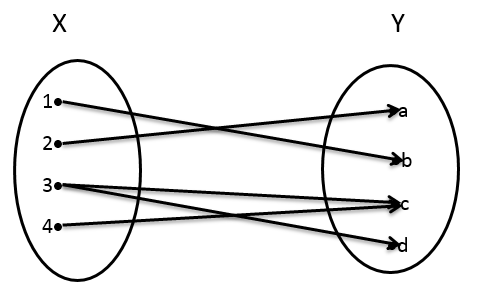
\includegraphics{hinh1}

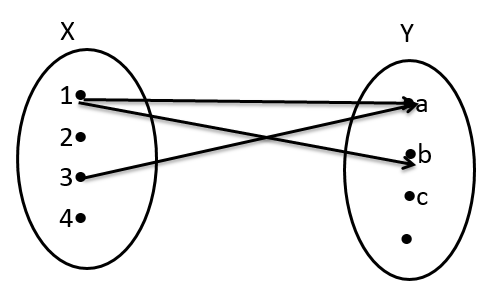
\includegraphics{hinh2}
\subsection{	Điều kiện xác định một ánh xạ.}
Để quy tắc $f:X\to Y$ là một ánh xạ thì phải thỏa mãn hai điều kiện sau:

\textbf{Điều kiện 1:} Quy tắc f xác định khắp nơi nghĩa là với mỗi $x\in X$ phải có ảnh y tương ứng thuộc Y.

\textbf{Điều kiện 2: } Quy tắc f đơn trị nghĩa là với mỗi $x\in X$ chỉ có tương ứng một phần tử y thuộc Y.

\textbf{Ví dụ.}

1) Quy tắc 

\centerline{\fullfunction{f}{\mathbb{R}}{\mathbb{R}}{x}{y=2x+1}}


Là một ánh xạ vì 

+)  Với mọi $x\in R$  luôn tồn tại $y=2x+1 \in R.$

+)  Với mỗi $y\in R$ sẽ có tương ứng một phần tử $x=\frac{(y-1)}{2} \in R.$

\textbf{1) Quy tắc }

\centerline{\fullfunction{f}{\mathbb{N}}{\mathbb{R}}{x}{y=\sqrt{x}}}


Không là một ánh xạ vì: Quy tắc $f$ không đơn trị.

Ví dụ với $x=9\in N$ sẽ tồn tại hai giá trị của y là: $y=3$ và $y=-3\in \mathbb{R}.$

Các cách xác định một ánh xạ.

Để có một ánh xạ $f:X\to Y$ người ta sử dụng những cách sau:

\textbf{Cách 1: }Cho ánh xạ dưới dạng biểu thức giải tích.

\textbf{Ví dụ.}
Ánh xạ: $f:\mathbb{R}\to \mathbb{R}$
\[x \mapsto \left\{ \begin{array}{l}
2x - 3\;\;\;\text{(Nếu x<0)}\\
\sin 3x \;\; \text{(Nếu } 0\le x <1 )\\
\log x + 5 \;\; \text{(Nếu } x\ge 1)
\end{array} \right.\]

\textbf{Cách 2:} Cho bằng bảng tương ứng giữa các giá trị của tập $X$ và tập $Y$.

Ví dụ.


\centerline{
\begin{tabular}{|c|c|c|c|}
    \hline
    X & 1 & 2 &3\\ \hline
   Y   & 6  & 7&8   \\ \hline
\end{tabular} } 
Xác định một ánh xạ 

\centerline{\fullfunction{f}{\mathbb{R}}{\mathbb{R}}{x}{y=x+5}}


\textbf{ Cách 3: }Cho ánh xạ dưới dạng biểu đồ.
Ví dụ.

+)  Biểu đồ phát triển dân số của tỉnh Vĩnh Phúc.

+)  Biểu đồ tăng hoặc giảm năng suốt lúa của các tỉnh đồng bằng sông Cửu Long.
 
 \subsection{Đồ thị của ánh xạ.}
\textbf{ Định nghĩa.}

     Cho ánh xạ $f:X\to Y$. Khi đó ta gọi tập  $G_f=\{(x,f(x))| x\in X\}\subset X\times Y$ là đồ thị của ánh xạ $f$.

Từ định nghĩa ánh xạ suy ra : Với mọi $x\in X$ tồn tại duy nhất  $y\in Y$ để $(x,y)\in G_f.$

Ví dụ.

Đồ thị hàm số 

\centerline{\fullfunction{f}{\mathbb{R}}{\mathbb{R}}{x}{3x+7}}


Là tập hợp $G=\{ (x,3x+7)  | x\in \mathbb{R}\}$. Khi biểu diễn G lên mặt phẳng tọa độ oxy ta được một đường thẳng không đi qua gốc tọa độ.

2) Cho $X=\{a,b,c\}, Y=\{1,2,3\} , f:X\to Y$ là ánh xạ xác định bởi         $f(a)=1,f(b)=2,f(c)=3$ thì đồ thị của $f$ là $G_f={(a,1),(b,2),(c,3)}$.

3) Cho hàm số  $y=f(x)$ . Khi đó biểu diễn đồ thị xác định bởi ánh xạ này trong mặt phẳng oxy chính là đồ thị của hàm số mà chúng ta đã biết.
Chẳng hạn: Đồ thị hàm số 

\centerline{\fullfunction{f}{\mathbb{R}}{\mathbb{R}}{x}{y=x^2-2x+4}}

Là tập $G=\{(x,x^2-2x+4)|x\in \mathbb{R}\}$. Khi biểu diễn G lên mặt phẳng tọa độ oxy ta được một parabol nằm phía trên trục hoành và tiếp xúc với trục hoành tại điểm $x=2$.

 \subsection{Hai ánh xạ bằng nhau.}
\textbf{ Định nghĩa.}

    Hai ánh xạ f và g được gọi là bằng nhau nếu chúng có cùng một tập đích và cùng quy tắc đặt tương ứng.
    
    Hay nói cách khác hai ánh xạ f và g bằng nhau nếu:
    
        $f:X\to Y ;  g:X\to Y$ và $f(x)=g(x)$ vói $x\in X$.
        
Ví dụ. Cho hai ánh xạ.

\fullfunction{f}{\mathbb{R}}{\mathbb{R}}{x}{f(x)=x^3-1} và \fullfunction{g}{\mathbb{R}}{\mathbb{R}}{x}{g(x)=(x-1)(x^2-x+1)}

Là hai ánh xạ bằng nhau.

\fullfunction{f}{\mathbb{R}}{\mathbb{R}}{x}{x^2} và \fullfunction{g}{\mathbb{R}}{[0;+\infty)}{x}{x^2}

Là hai ánh xạ không bằng nhau vì chúng có tập đích khác nhau.

\subsection{Thu hẹp và mở rộng ánh}
 Định nghĩa.
Gỉa sử $f:X\to Y$ là một ánh xạ và $A$ là một bộ phận của $X$. Ta gọi ánh xạ

\centerline{\fullfunction{g}{A}{Y}{x}{g(x)=f(x)}}

Gọi là cái thu hẹp của $f$ vào bộ phận  A, kí hiệu là $g=f/A$, còn ánh xạ $f$  gọi là cái mở rộng của g trên tập $X$.

Ví dụ: Cho các ánh xạ

\fullfunction{f}{\mathbb{R}}{\mathbb{R}}{x}{f(x)=\cos x}

\fullfunction{g}{\left[-\frac{\pi}{2};\frac{\pi}{2} \right ]}{\mathbb{R}}{x}{g(x)=\cos x}
        
\fullfunction{h}{\mathbb{R}}{[-1,1]}{x}{h(x)=\cos x}

\fullfunction{k}{\left[-\frac{\pi}{2};\frac{\pi}{2} \right ]}{[-1,1]}{x}{k(x)=\cos x}

Bốn ánh xạ này không bằng nhau vì các tập nguồn và các tập đích của chúng khác nhau. Chúng trùng nhau trên $X=\left[-\frac{\pi}{2};\frac{\pi}{2} \right ]$ và $Y=[-1,1]$. Ta không đồng nhất chúng,  nhưng kí hiệu giá trị chung của chúng tại x là cosx

         g là thu hẹp của f vào $\left[-\frac{\pi}{2};\frac{\pi}{2} \right ]$
         
         k là thu hẹp của h vào $\left[-\frac{\pi}{2};\frac{\pi}{2} \right ]$
         
         h được cảm sinh bởi f bằng cách thu hẹp đích vào $[-1,1]$
         
         k được cảm sinh bởi g bằng cách thu hẹp đích vào $[-1,1]$
         
\textbf{Nhận xét:} Có duy nhất một ánh xạ thu hẹp của một ánh xạ đã cho, song có rất nhiều ánh xạ mở rộng của một ánh xạ đã cho.

\section{Ảnh và tạo ảnh}
\subsection{Định nghĩa}
Cho ánh xạ \fullfunction{f}{X}{Y}{x}{y=f(x)}

$f(x)$ là ảnh của x bởi f hay giá trị của ánh xạ f tại điểm x.

$A\subset X$, tập $f(A)=\{y\in Y|$ tồn tại $x\in A$ sao cho $f(x)=y\}$ được gọi là tập ảnh của tập con A qua ánh xạ $f$.

$B\subset Y$, tập $f^{-1} (B)=\{x\in X| f(x)\in B\}$ được gọi là tập tạo ảnh toàn phần của tập con B qua ánh xạ $f$.

Tập hợp $f(x)\subset Y$ gọi là ảnh của ánh xạ f, kí hiệu $Imf$.

\textbf{Ví dụ.}

1) Cho hai tập hợp $X=\{a,b,c,d,e\}$ và $Y=\{1,2,3,4,5,6\}$ và ánh xạ $f:X\to Y$ xác định bởi bảng sau:

\begin{tabular}{|c|c|c|c|c|c|}
    \hline
    x & a & b&c&d&e \\ \hline
    f(x)  & 1   & 3&2&5&1   \\ \hline
\end{tabular}
 
Ánh xạ f được biểu diễn bởi lược đồ như hình vẽ:

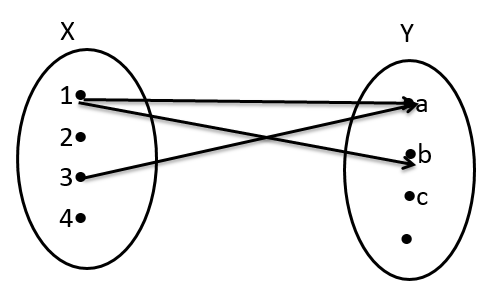
\includegraphics{hinh2}

Cho hai tập con A,B của $X: A=\{a,b,e\}$  và $B=\{c,d\}$, ảnh của A và B qua ánh xạ f là: $f(A)=\{1,3\} ; f(B)=\{2,5\}.$

Tạo ảnh của $C=\{1,3,5\}$  và $D=\{2,4,6\}$ qua ánh xạ $f$ là:

$ f^{-1} (C)=\{a,e,b,d\}$  và $f^{-1} (D)=(c).$

2) Giả sử \fullfunction{f}{\mathbb{R}}{\mathbb{R}}{x}{y=f(x)=x^2}

Tập $A=\{2,3,7\}$ và $R^-$  là tập hợp các số thực không dương

 $R^-=\{x\in R | x\le 0\}$
 
 Khi đó $f(A)=\{4,9,49\}$  và $f(R^- )=R.$
 
$f^{-1} (\mathbb{R}^- )=\phi$

\subsection{Các tính chất cơ bản.}
         Cho ánh xạ $f:X\to Y$.  $A,B$ là các tập hợp con của $X; C,D$ là các tập hợp con của Y. Khi đó :
         
+ ảnh của một tập hợp rỗng là một tập hợp rỗng

   $A=\varnothing \Leftrightarrow $ thì $f(A)=\varnothing$
   
+ Ảnh của tập hợp con là tập hợp con của ảnh

   $A\subset B \Rightarrow f(A)\subset f(B)$
   
+ Ảnh của phần giao nằm trong giao của phần ảnh

   $f(A \cap B)\subset f(A)\cap f(B)$
   
+ Ảnh của các phần hợp là hợp của các phần ảnh

$f(A\cap B)=f(A)\cap f(B) $

+ Tạo ảnh toàn phần của phần hợp là phần hợp của các tạo ảnh toàn phần

 $ f^{-1} (C \cup D)=f^{-1} (C)\cup f^{-1} (D)$
 
+ Tạo ảnh toàn phần của phần giao là giao của các tạo ảnh toàn phần

$f^{-1} (C \cap D)=f^{-1}(C) \cap f^{-1} (D)$

\section{Các ánh xạ đặc biệt.}
\subsection{Đơn ánh}
\textbf{Định nghĩa }
Ánh xạ: \fullfunction{f}{X}{Y}{x}{y=f(x)} được gọi là một đơn ánh nếu thỏa mãn. 

Với $\forall x_1,x_2\in X: x_1\neq x_2\Leftarrow f(x_1)\neq f(x_2)$

Hoặc $\forall x_1,x_2:f(x_1 )=f(x_2 )\Leftarrow x_1=x_2$

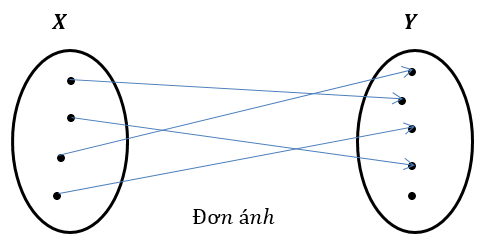
\includegraphics{hinh4}

\textbf{Ví dụ.}
Xét ánh xạ :

\fullfunction{f}{\mathbb{R}}{\mathbb{R}}{x}{x^3}

Rõ ràng f là đơn ánh vì nếu x,y là những số thực thì quan hệ $x^3=y^3$ kéo theo $x=y$.

Ánh xạ \fullfunction{f}{\mathbb{R}}{\mathbb{R}}{x}{y=x^4}

Không phải là đơn ánh .

Thật vật:  với mọi $x_1,x_2\in R$, nếu $f(x_1 )=f(x_2) \Leftrightarrow  x_1^4=x_2^4$

$\Rightarrow x_1=\pm x_2 $
Do đó f không là đơn ánh.

\subsection{Toàn ánh}
\textbf{Định nghĩa}

Ánh xạ \fullfunction{f}{X}{Y}{x}{y=f(x)} được gọi là toàn ánh nếu thỏa mãn
          
$\forall y\in Y,\exists x\in X$ sao cho $y=f(x)$  hoặc tương ứng với nó là $f(X)=Y$

Người ta còn gọi một toàn ánh $f:X\to Y$ là một ánh xạ từ $X$ lên $Y$

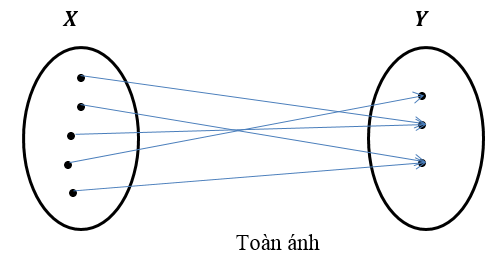
\includegraphics{hinh5}

\textbf{Ví dụ.}

Ánh xạ \fullfunction{f}{\mathbb{R}^+}{\mathbb{R^+}}{x}{x^4}

Là song ánh.

Thật vậy.

+) Chứng minh $f$ là toàn ánh.

Xét phương trình (ẩn x): $y=x^4, y\in \mathbb{R}^+$

phương trình này có nghiệm duy nhất $x=\sqrt[4]{y}, y\in \mathbb{R^+}$
do đó $f$ là toàn ánh.

+) chứng minh $f$ là đơn ánh.

Với mọi $x_1,x_2\in \mathbb{R}^+$, nếu $f(x_1 )=f(x_2 )\Leftrightarrow x_1^4=x_2^4$

$\Rightarrow x_1=x_2$

Do đó $f$ là đơn ánh.

Vậy $f$ là song ánh.

\textit{Chú ý: Một cách tương đương, ta có thể định nghĩa đơn ánh, toàn ánh và song ánh như sau:}

    + Ánh xạ f là đơn ánh nếu mọi $y=f(x)$ có không quá một tạo ảnh x thuộc X, hay phương trình ẩn x: $f(x)=y$ vô nghiệm hoặc có một nghiệm duy nhất với mọi y thuộc Y.
    
    + Ánh xạ f là toàn ánh nếu mọi y thuộc Y đều có ít nhất một tạo ảnh x thuộc X hay phương trình ẩn x, $f(x)=y$ luôn có nghiệm với mọi y thuộc Y.
    
    + Ánh xạ f là song ánh nếu mọi y thuộc Y có một và chỉ một tạo ảnh x thuộc X, Hay phương trình ẩn x, $f(x)=y$ luôn có một nghiệm duy nhất với mọi y thuộc Y.

\section{Tích các ánh xạ.}
\subsection{Định nghĩa.}

Cho ánh xạ $f: \mathbb{X}\to \mathbb{Y}$ và ánh xạ g: $\mathbb{Y}\to \mathbb{Z}$

Ánh xạ  

 \centerline{ \fullfunction{h}{X}{Z}{x}{g(f(x))}}

Gọi là tích của ánh xạ g và ánh xạ f. Kí hiệu $g_o f$ hay $gf.$

Như vậy $gf:X\to Z$ và $\forall x\in X,(gf)(x)=g(f(x)),D_gf=D_f$  và $R_gf=R_g$

\emph{ Chú ý:} Để tồn tại tích $gf$ thì miền giá trị của ánh xạ $f$ phải trùng với miền xác định của ánh xạ g, như thế có thể không tồn tại $fg$. Ngay cả khi tồn tại gf và fg nhưng nói chung $gf\neq fg$. Nghĩa là tồn tại khi và chỉ khi $R_f \subseteq D_g$

\textbf{Ví dụ.} Cho hai ánh xạ 
\begin{align*}
f: x\mapsto \frac{1}{x^2}, x\in \mathbb{R}\\
D_f=(-\infty,0),R_f=(0,+\infty)
\end{align*} 
và ánh xạ 
\begin{align*}
g: x\mapsto 2x+1, x\in \mathbb{R}\\
D_f=\mathbb{R}, R_g=\mathbb{R}
\end{align*} 

+) Xét $gf.$

  Ta có: $R_f=(0,\infty) \subseteq R=D_g$.Do đó $gf$ tồn tại
  
   $(gf)(x)=g(f(x))=g(\frac{1}{x^2})=2(\frac{1}{x^2})+1$
   
   $\Rightarrow gf:x\mapsto \frac{2}{x^2}+1,x\in \mathbb{R}^-$
   
   $D_gf=\mathbb{R}^-,   R_gf=(1,\infty)$
   
+) Xét $fg$.

   Ta có: $R_g=R \nsubseteq (-\infty,0)=D_f$. Do đó $fg$ không tồn tại.
   
    Để $fg$ tồn tại thì $R_g\subset D_f\Leftrightarrow 2x-1\le 0
     \Leftrightarrow x\le \frac{-1}{2}$

 Vậy với $g_R:x\to 2x+1,x\in R,x\le \frac{-1}{2}$  thì $fg_R$  tồn tại.

\subsection{Một số tính chất}

\textbf{Định lí 1:}

Tích các ánh xạ có tính chất kết hợp. Tức là với mọi ánh xạ $f:X\to Y, g:Y\to Z,h: Z\to V$  ta có $(hg)f=h(fg).$

\textbf{Định lí 2:}

a) Tích của hai đơn ánh là một đơn ánh.

b) Tích của hai toàn ánh là một toàn ánh (nếu các tích trên xác định)
Đặc biệt tích của hai song ánh là song ánh.

\textbf{Định lí 3:}

a) Nếu $gf$ là đơn ánh thì f là đơn ánh.

b) Nếu $gf$ là toàn ánh thì g là toàn ánh.

\section{Ánh xạ ngược.}
\subsection{Định nghĩa.}
      Cho ánh xạ $f:X\to Y$. Nếu có ánh xạ $g:Y\to X$ sao cho $gf=1_X$  và $fg=1_Y$

Thì g được gọi là ánh xạ ngược của f.

Ánh xạ ngược của f(nếu có) được kí hiệu là $f^{-1}$

Ta có $f^{-1} f=I_X,ff^{-1}=I_Y$

Từ định nghĩa ta có:

 +) Nếu f có ánh xạ ngược $f^{-1}$ thì $f^{-1}$ cũng có ánh xạ ngược  và $(f^{-1} )^{-1}=f.$
 
 +) Nếu $f:X\to Y$ và $g:Y\to Z$ đều có ánh xạ ngược thì $gf:X\to Z$ cũng có ánh xạ ngược và $(gf)^{-1}=f^{-1} g^{-1}$.

 +) Ánh xạ đồng nhất $1_X:X\to Y$ có ánh xạ ngược $1_X^{-1}=1_X.$

\subsection{Các ví dụ.}
a)	Ánh xạ \fullfunction{f}{\mathbb{R}}{\mathbb{R}}{x}{2x+1} có ánh xạ ngược là

 \fullfunction{g}{\mathbb{R}\to \mathbb{R}}{x}{\frac{1}{2}x-\frac{1}{2}}


Thật vậy $$\forall x\in \mathbb{R}:(gf)(x)=g(f(x))=g(2x+1)=\frac{1}{2} (2x+1)-\frac{1}{2}$$
 $$=x+\frac{1}{2}-\frac{1}{2}=x=I_R (x)\Rightarrow gf=I_R$$
Mặt khác:
$$\forall x\in R:f(g(x))=f(\frac{1}{2} x-\frac{1}{2})=2(\frac{1}{2} x-\frac{1}{2})+1\Rightarrow fg=I_R$$

b)	Ánh xạ \fullfunction{f_{m.n}}{mZ}{nZ}{ma}{na} có ánh xạ ngược là:
   
\fullfunction{f_{n.m}}{nZ}{mZ}{na}{ma}

Với $m,n \in \mathbb{N}^*$

\subsection{Điều kiện có ánh xạ ngược.}
Ánh xạ $f:X\to Y$ có ánh xạ ngược khi và chỉ khi $f$ là song ánh.
Chứng minh.

$\Rightarrow ]$ Giả sử $f:X\to Y$ có ánh xạ ngược là $g:Y\to X$

Khi đó $gf=1_X$  là đơn ánh $\Rightarrow f$ là đơn ánh

Và  $fg=1_Y$ là toàn ánh $\Rightarrow f$ là toàn ánh

Kết hợp lại ta có $f$ là song ánh.
$\Leftarrow ]$ ngược lại cho $f:X\to Y$ là song ánh ta xác định quy tắc $g:Y\to X$ như sau:

Biến $y\in Y$ thành $x\in X$ sao cho $y=f(x)$. Do $f$ là song ánh nên $g$ là ánh xạ.
Mặt khác:

$\forall x\in X,(gf)(x)=g(f(x))=g(y)=x=1_X (x) \Rightarrow gf=1_X$

$\forall y\in Y,(gf)(y)=f(g(y))=f(x)=y=1_Y (y)\Rightarrow fg=1_Y$

\subsection{Quy tắc tìm ánh xạ ngược.}
   \emph{Bước 1: }Kiểm tra xem ánh xạ $f:X\to Y$ có phải là song ánh hay không ?
   
  \emph{ Bước 2: }Xét phương trình $f(x)=y$ ta tìm được $x=g(y)$. Khi đó xác định ánh xạ $g:Y\to X$ là ánh xạ ngược cần tìm.
   
Ví dụ.

a)	Xét hàm số bậc nhất $y=ax+b,   a,b\in \mathbb{R},a\neq 0$ được xem là ánh xạ 

 %hinh parapol
\begin{wrapfigure}{r}[0pt]{0.25\linewidth}

    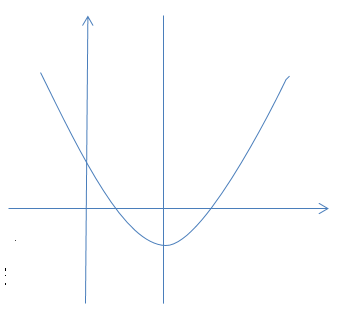
\includegraphics[scale=0.5]{hinh6}
\end{wrapfigure}

\fullfunction{f}{\mathbb{R}}{\mathbb{R}}{x}{ax+b}

     Kiểm tra thấy ngay f là song ánh $\Rightarrow f$ có ánh xạ ngược.
     
     Xét phương trình $f(x)=y \Leftrightarrow ax+b=y\Rightarrow x=\frac{y-b}{a}$

     Tức là $g(y)=\frac{y-b}{a}=\frac{1}{a}-\frac{b}{a}$

     Hay $g(x)=\frac{1}{a}-\frac{b}{a}$  lại là hàm số bậc nhất.

b) Xét hàm số bậc hai $y=ax^2+bx+c,a,b,c\in R,a\neq 0.$

Giả sử $a>0$, giả sử đồ thị có dạng:

     Được xem là ánh xạ \fullfunction{f}{\mathbb{R}}{\mathbb{R}}{x}{ax^2+bx+c}
           
 +) $f$ không là đơn ánh vì :
Chọn $x_1=\frac{-b}{2a}+\alpha ,x_2=\frac{-b}{2a}-\alpha ,\alpha>0$

Ta lại có $x_1\neq x_2$  nhưng $f(x_1 )=f(x_2)$

 +) $f$ không là toàn ánh vì:
 
$\forall y< \frac{-\Delta}{4a}$ thì phương trình $ax^2+bx+c=y$ vô nghiệm 

-Từ hàm số bậc hai ta có thể xây dựng hàm số mới là song ánh.
Thật vậy.

Xét ánh xạ \fullfunction{g}{\left[-\frac{b}{2a},+\infty \right ) }{ \left[-\frac{\Delta}{4a} ,+\infty \right )}{x}{ax^2+bx+c}


+) kiểm tra được g là song ánh

+) tìm ánh xạ ngược của g

Xét phương trình $g(x)=y với y\in \left[\frac{-\Delta}{4a},+\infty \right )$

$\Leftrightarrow ax^2+bx+c=y$

$\Leftrightarrow ax^2+bx+(c-y)=0$

Có $\Delta_1=b^2-4a(c-y)=b^2-4ac+4ay=\Delta+4ay$

$y>\frac{-\Delta}{4a}\Rightarrow 4ay>-\Delta \Rightarrow \Delta -\Delta =0$

Do đó phương trình bậc hai trên có hai nghiệm

$$x_{1,2}=\frac{-b\pm \sqrt{\Delta_1}}{2a}=-\frac{b}{2a}\pm \frac{\sqrt{\Delta_1}}{2a}$$

Do $x\in \left[-\frac{b}{2a},+\infty \right )\Rightarrow $ chỉ lấy giá trị $x_1=\frac{-b}{2a}+\frac{\sqrt{\Delta_1}}{2a}$

Và có hàm số ngược là :$g^{-1}(y)=\frac{-b}{2a}+\frac{\sqrt{b^2-4a(c-y)}}{2a}$

Hay hàm số $y=\frac{-b}{2a}+\frac{\sqrt{b^2-4a(c-x)}}{2a}$

Chú ý: Đồ thị của  hàm số f và $f^{-1}$ đối xứng nhau qua đường thẳng $y=x$. Gọi H là đồ thị của ánh xạ $f. H^{-1}$ là đồ thị của ánh xạ $f^{-1}$. Khi đó $(a,b)\in H \Leftrightarrow (b,a)\in H^{-1}$.

c) Cho ánh xạ $f:x\mapsto 2x+4,x\in \mathbb{R},x>0$.Tìm $f^{-1}$?
Xét ánh xạ $f:x\mapsto 2x+4,x\in R,x>4$

Ta có $D_f=(0,\infty),R_f=(4,\infty)$

+) kiểm tra tính song ánh của f.

$\forall x_1,x_2\in (0,\infty)$ .Giả sử $f(x_1 )=f(x_2 )$

$\Leftrightarrow 2x_1+4=2x_2+4\Leftrightarrow 2x_1=2x_2\Leftrightarrow x_1=x_2$

Vậy f là đơn ánh   (1)

$\forall y=2x+4\in (4,\infty),\exists x\in (0,\infty)$  thỏa mãn $f(x)=2x+4=y$

Vậy $f$ là toàn ánh  (2)

Từ (1) và (2) ta có $f$ là song ánh nên $f$ có ánh xạ ngược.

Đặt $f(x)=y \Rightarrow 2x+4=y\Leftrightarrow 2x=y-4\Leftrightarrow x=\frac{y-4}{2}$

$f^(-1) (y)=x \Rightarrow f^{-1} (y)=\frac{y-4}{2}$

$\Rightarrow f^{-1} (x)=\frac{x-4}{2}$

Vậy $f^{-1}:x\mapsto \frac{x-4}{2},x\in \mathbb{R},x>3 , D_(f^{-1} )=(4,\infty)$ và $R_(f^(-1) )=(0,\infty)$

\section{Phép toán hai ngôi.}

\subsection{Định nghĩa}
Cho $X$ là một tập hợp không rỗng. Ta gọi là một phép toán hai ngôi trên tập hợp $X$ một ánh xạ f từ tập hợp $X\times X$ đến tập hợp $X$
                                      $$ f:X\times X\to X$$
 Ánh xạ này cho tương ứng với mỗi cặp $(a,b)\in X\times X$ một phần tử $c\in X$ hoàn toàn xác định; phần tử c này được gọi là hợp thành của các phần tử a và b bởi phép toán hai ngôi $f$. Nó chính là ảnh của phần tử $(a,b)\in X\times  X$ qua ánh xạ $f$:

$(a,b)\in X\times X\mapsto c=f(a,b)=X$

Kí hiệu $T(x,y)$

\textbf{Ví dụ.}

Trong tập hợp N các số tự nhiên phép cộng, phép nhân là những phép toán hai ngôi; cái hợp thành của $a\in \mathbb{N}$ và $b\in \mathbb{N}$ bởi các phép toán đó kí hiệu theo thứ tự bằng $a+b,ab$. Phép hợp thành $a^b $là một phép toán hai ngôi trong tập $\mathbb{N}^*=\mathbb{N}-\{0\}.$

Phép trừ không  phải là phép toán hai ngôi trong N, nhưng là một phép toán hai ngôi trong tập Z các số nguyên.

Trong tập hợp $ \mathbb{N}^*$, phép nâng lũy thừa $a^n$ là một phép toán hai ngôi, nhưng phép chia không phải là phép toán hai ngôi.
Tương ứng

$$(a,n)\mapsto a^n$$

Với $a,b\in  \mathbb{N}^*$, xác định một ánh xạ từ $\mathbb{N}^*\times \mathbb{N}^*$  đến $N^*$.   
   
Nhưng tương ứng $(a,b)\mapsto a:b$     

 Với $a,b \in  \mathbb{N}^*$, không xác định  một ánh xạ từ $\mathbb{N}^*\times \mathbb{N}^*$  đến $\mathbb{N}^*. $  

\subsection{Các tính chất thường gặp ở phép toán hai ngôi}
Giả sử T là một phép toán trong tập hợp X.
	Tính chất kết hợp: $\forall x,y,z\in X:(xTy)Tz=xT(yTz)$
	
	Tính chất giao hoán: $\forall x,y\in X:xTy=yTx$
	
	Tính chất phân phối: $\forall x,y,z\in X:xT(y*z)=(xTy)*(xTz)$
	
   $\forall x,y,z\in X:(y*z)Tx=(yTx)*(zTx)$   
    
\textbf{Ví dụ.} trong N, phép cộng và phép nhân có tính chất kết hợp, giao hoán; phép nhân phân phối đối với phép cộng.

Ta có:

+) a+(b+c)=(a+b)+c

+) a(bc)=(ab)c

+) a+b=b+a

+) ab=ba

+  a(b+c)=ba+bc

Với mọi a,b,c thuộc N.

\subsection{Số tự nhiên .}
\textbf{a.Bản số}

Mỗi tập hợp có một bản số, sao cho hai tập hợp tương đương có cùng một 
bản số.

bản số của tập hợp A kí hiệu là $Card(A)$. 

Vậy theo định nghĩa:
  $Card(A)=Card(B)\Leftrightarrow A\sim B$
  
\textbf{b.Số tự nhiên.}

Bản số của một tập hợp hữu hạn được gọi là một số tự nhiên.
      
Tập hợp tất cả các số tự nhiên được kí hiệu là N. như vậy $a\in N$ khi và chỉ khi tồn tại một tập hợp hữu hạn A sao cho $a=Card(A).$

Ví dụ.

$\O$ là một tập hợp hữu hạn, bản số của nó là một số tự nhiên gọi là số không: $Card(\O )=0.$

\textbf{c. Các phép toán trên N.}

Cho a,b là các số tự nhiên, gọi A,B là các tập hợp mà $a=Card(A), b=Card(B)$  và $A \cap B= \O $.

-Phép cộng:

$\mathbb{N}\times N\to \mathbb{N}$

$(a,b)\mapsto a+b=Card(A\cup B)$
   
-Phép nhân:

$\mathbb{N}\times N\to \mathbb{N}$

$(a,b)\mapsto a.b=Card(A\times B)$
   
Dựa vào các tính chất của phép toán hợp và tích đề-các của các tập hợp ta suy ra tính chất của phép cộng và nhân các số tự nhiên:

\textbf{Tính chất của phép cộng.}

Phép cộng có tính chất giao hoán: $a+b=b+a$

Phép công có tính chất kết hợp: $(a+b)+c=a+(b+c)$

Số 0 là phần tử trung hòa: $0+a=a.$

Phép cộng có tính chất giản ước được: $a+b=a+c$ kéo theo $b=c.$

\textbf{Tính chất của phép nhân.}

Phéo nhân có tính chất giao hoán:$ab=ba$

Phép nhân có tính chất kết hợp: $a(bc)=(ab)c$

Số 1 là phần tử trung hòa: $1.a=a$

\textbf{Tính chất giữa phép nhân và phép công.}

$a(b+c)=ab+ac$

Một số bài tập liên quan.

\textbf{Bài 1:} các quy tắc sau có phải là ánh xạ không? Tại sao?

a) \fullfunction{f}{\mathbb{R}}{\mathbb{R}}{x}{2x+3}

b) \fullfunction{g}{\mathbb{R}}{\mathbb{R}}{x}{\frac{1}{x^2}}

Giải.

a) $f$ là ánh xạ vì $f$ thỏa mãn hai điều kiện là f xác định khắp nơi và f có tính đơn trị.

Thật vậy:
$f$  xác định khắp nơi vì: $\forall x\in \mathbb{R}$ luôn tồn tại $y=2x+3\in \mathbb{R}.$

$f$ đơn trị vì với mỗi $y\in \mathbb{R}$ sẽ có tương ứng một phần tử $x=\frac{y-3}{2}\in \mathbb{R}$.

$g$ không phải là ánh xạ vì với $x=0$ thì  $\frac{1}{x^2}$   không có nghĩa.

\textbf{Bài 2: }lập tất cả các tương ứng giữa tập hợp $X=\{a,b\}$ và tập $Y=\{1\}$. Hãy chỉ ra những tương ứng nào trong các tương ứng đó là ánh xạ từ tập hợp $X$ đến tập hợp $Y$.

Giải.

Các tương ứng giữa $X$ và $Y$ là $f=\{(a,1),(b,1)\}  ;g=\{(a,1)\}  ;h=\{(b,1)\}$

Tương ứng $f$ là ánh xạ từ $X$ đến $Y$ vì thỏa mãn định nghĩa của ánh xạ: Mọi phần tử trong X đều có ảnh trong Y và ảnh đó là duy nhất.

\textbf{Bài 3:} Xét tính đơn ánh, toàn ánh, song ánh của các ánh xạ sau. Trường hợp f là song ánh hãy tìm ánh xạ ngược của nó.

a) \fullfunction{f}{\mathbb{R}}{\mathbb{R}}{x}{x^3-1}

b) \fullfunction{f}{\mathbb{R}}{\mathbb{R}}{x}{x^2-5x+6}

c) \fullfunction{f}{\mathbb{R}\setminus \{1\}}{\mathbb{R}}{x}{\frac{2x+3}{x-1}}

d) \fullfunction{f}{[1,+\infty)}{[-5,+\infty)}{x}{x^2-2x-4}

Giải.
a)
$\forall x_1,x_2\in R,x_1\neq x_2 \Rightarrow x_1^3-1\neq x_2^3-1 \Rightarrow f(x_1 )\neq f(x_2 )$. Vậy $f$ là đơn ánh.

$\forall y\in \mathbb{R}, \exists x=\sqrt[3]{(y+1)}$  để $f(x)=y$. Vậy f là toàn ánh.

Do đó f là song ánh và có ánh xạ ngược của f là \fullfunction{f^{-1}}{\mathbb{R}}{\mathbb{R}}{x}{ \sqrt[3]{(x+1)}}


b) $f(3)=f(2)=0\Rightarrow f$ không đơn ánh; $f^(-1) (-3)=\O \Rightarrow f$ không toàn ánh.

c) Xét phương trình ẩn x: $\frac{2x+3}{x-1} =y \Rightarrow y(x-1)=2x+3\Rightarrow (y-2)x=3+y$

nếu $y\neq 2$ thì phương trình có một nghiệm duy nhất

nếu $y=2$ thì phương trình vô nghiệm

Do đó $f$ là đơn ánh nhưng không toàn ánh.

d) Phương trình $x^2-2x-4=y,\forall y\in [-5,+\infty)$  có hai nghiệm là $1\pm \sqrt{y+5}$, nhưng chỉ có $1+\sqrt{y+5}\in [1,+\infty)$, do đó $f$ là song ánh.

\textbf{Bài 4: } Cho ánh xạ \fullfunction{f}{\mathbb{R}}{\mathbb{R}}{x}{x^2-5x+1}

Hãy xác định:

a) $f(0),f(1),f(-3)$

b) $f^{-1} (1),f^{-1} (-3)$

c) $f^{-1} ([-3,1])$

Giải.

a) $f(0)=0^2-5.0+1=1,f(1)=-3,f(-3)=25$

b) $f^(-1) (1)=\{x\in \mathbb{R}| x^2-5x+1=1\}=\{0,5\}$

c) $f^{-1} (-3)=\{x\in R|x^2-5x+1=-3\}=\{-1;-4\}$

d) $f^{-1} ([-3,1])=\{x \in \mathbb{R} |-3\le x^2-5x+1\le 1\}=[0,5]$

\textbf{Bài 5: }Tìm hàm số ngược của các hàm số sau:

a) $y=\frac{2x+1}{x-1}$  xác định trên tập hợp $\mathbb{R}$.

b) $y=-4x^2$  xác định trong khoảng $(-\infty,0)$

Giải.

$y=\frac{2x+1}{x-1} \Rightarrow y(x-1)=2x+1\Rightarrow yx-y=2x+1$

$\Rightarrow yx-2x=y+1\Rightarrow x(y-2)=y+1$

với $y\neq 2$ ta có $x=\frac{y+1}{y-2}$. Thay $x$ bởi $y,y$ bởi $x$ ta có $y=\frac{x+1}{x-2}$

Vậy hàm số ngược của hàm số $y=\frac{2x+1}{x-1}$ xác định trên $R\setminus {1}$ là $y=\frac{x+1}{x-2}$xác định trên $\mathbb{R}\setminus{2}$

b) $y=-4x^2\Rightarrow x^2=\frac{-y}{4} \Rightarrow x=-\sqrt{\frac{-y}{4}}$  (vì $x<0$)

Thay x bởi $y, y$ bởi x ta có $y=-\sqrt{\frac{-x}{4}}$

Vậy hàm số ngược của $y=-4x^2$  xác định trong khoảng $(-\infty,0)$ là $y=- \sqrt{\frac{-x}{4}}$ xác định trong khoảng $(-\infty,0)$ .

\textbf{Bài 6: } cho $A=B={a,b,c};C={1,2,3},g:A\to B$ và $f:B\to C$  được cho như sau:

$g(a)=b,g(b)=c,g(c)=a$

$f(a)=3,f(b)=2,f(c)=1$

Hãy xác định ánh xạ hợp $f_o g$ của ánh xạ $f$ và $g$, ánh xạ $g_o f$ của ánh xạ $g$ và $f$.

Giải.

Ta có: 
$f_0 g:A\to C$ được xác định như sau

$(f_o g)(a)=f(g(a))=f(b)=2$  

$(f_o g)(b)=f(g(b))=f(c)=1$

$(f_o g)(c)=f(g(c))=f(a)=3$

ánh xạ $g_o f$ không xác định  vì tập ảnh của f không là tập con của tập xác định của $g$.

\textbf{Bài 7:} Cho $f: \mathbb{Z}\to  \mathbb{Z}$ và $g: \mathbb{Z}\to \mathbb{Z}$ là hai ánh xạ xác định trên tập số nguyên và lấy giá trị nguyên, cho bởi công thức sau:
$f(n)=n-1\;\;\;\;\;\;\;\;\; g(n)=3n+1$

Hãy xác định các hàm số hợp $f_o g$ của ánh xạ $f$ và g,ánh xạ $g_o f$ của $g$ và $f$

Giải.

Hàm số hợp $f_o g:\mathbb{Z}\to \mathbb{Z}$  được xác như sau:

$$(f_o g)(n)=f(g(n))=f(3n+1)=3n+1-1=3n$$

 Hàm số hợp $g_o f:\mathbb{Z}\to \mathbb{Z}$  được xác như sau:

$$(g_o f)(n)=g(f(n))=g(n-1)=3(n-1)+1=3n-2.$$



\chapter{NỘI DUNG TOÁN HỌC Ở PHỔ THÔNG CÓ LIÊN QUAN ĐẾN ÁNH XẠ.}
\section{Ánh xạ trong toán tiểu học}
\medskip
    Nội dung môn Toán ở Tiểu học được trình bày dưới ánh sáng các tư tưởng của toán học cao cấp, toán học hiện đại nên hầu hết các nội dung toán Tiểu học đều có mối liên hệ với nội dung dạy học tập hợp, ánh xạ ở đại học. Việc hình thành các khái niệm toán học ở tiểu học như số tự nhiên, các phép toán trên tập các số tự nhiên (phép cộng, phép trừ các số tự nhiên..) đều xuất phát từ các kiến thức của lý thuyết tập hợp, ánh xạ.
\medskip
    Sách giáo khoa lớp 1 đã vận dụng tư tưởng trên khi trình bày khái niệm số tự nhiên theo cách hiểu là số phần tử của một tập hữu hạn,Ví dụ  khi hình thành số 3, sách toán 1 sử dụng các mô hình biểu diễn dường cong khép kín (chỉ biểu đồ Ven minh họa cho một tập hợp, bên trong gồm 3 đồ vật (giống nhau) gần gũi với cuộc sống hàng ngày của học sinh(chỉ phần tử của tập hợp đó).
    
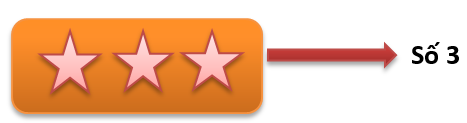
\includegraphics{hinh7}

\medskip
    Ngay từ những lớp đầu của bậc tiểu học, học sinh đã được làm quen với khái niệm ánh xạ một cách ẩn ngầm. Cơ sở lý thuyết tập hợp của việc dạy học khái niệm số tự nhiên ở tiểu học là sự “tương ứng” đó là sự tương ứng đơn giản giữa hai tập hợp: 3 ngôi sao, 3 mặt cười,  … tương ứng với số 3.\\

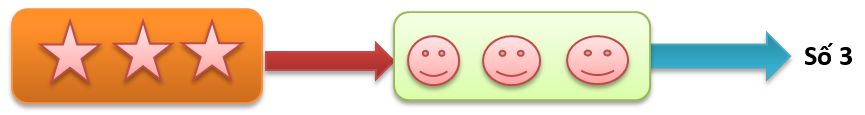
\includegraphics[scale=.6]{hinh8}

\medskip
Do học sinh chưa có khái niệm ánh xạ nên dùng những hình ảnh tương ứng cho học sinh dễ hiểu.

\medskip
 Những bài toán ở Tiểu học mô hình chung dựa vào tập hợp.
 
{\bf Ví dụ}

Tính nhanh:     $$941+748+174+671+826+252+59+329$$

 Cơ sở của ví dụ trên chính là định lý về tính chất giao hoán của phép toán hai ngôi.

Giải bằng kiến thức tiểu học

\begin{align*}
941+748+174+826+252+59 &=(941+59) + (748+252) + (174+826) \\ 
 &= 1000+1000+1000\\ 
 &= 3000
\end{align*}


Ở những lớp tiếp theo của bậc tiểu học, học sinh đã bước đâu làm quen với những bài toán đố, bài toán thực tế đơn giản. Cơ sở của những bài toán này chính là dựa vào kiến thức của ánh xạ.

{\bf Ví dụ}

An cùng mẹ đi chia kẹo cho các bạn nhỏ có hoàn cảnh khó khăn trong ngày quốc tế thiếu nhi . Ban đầu An chia cho Nam một nửa số kẹo của mình.Sau đó An chia cho $20$ bạn nhỏ tiếp theo mỗi bạn một chiếc kẹo thì An còn lại $5$ chiếc kẹo. Hỏi An có tất cả bao nhiêu chiếc kẹo?


    \textit{Giải bài toán bằng kiến thức toán cao cấp: Cơ sở của bài toán trên chính là ánh xạ}
    
\begin{align*}
\text{ \space}f:\mathbb{N}&\longrightarrow\mathbb{N}\\
x&\longmapsto y=f(x)=\frac{x}{2}-20
\end{align*}

\medskip
\textit{Giải bài toán bằng kiến thức tiểu học: Phương pháp giải chủ yếu cho các bài toán ở tiểu học chính là các phương pháp như: Tính ngược từ cuối lên, ứng dụng sơ đồ, dùng chữ số thay thế…}
\medskip
Từ lớp 4, SGK đã bắt đầu giới thiệu về các biểu thức chứa chữ đơn giản, các bài toán tìm $x$ hay tìm giá trị của biểu thức với 1 hoặc 2 biến.
 
 
{\bf Ví dụ}
\medskip
1.	Tính giá trị của biểu thức $7 \times x + 2$ với $x=1,2,3$

\medskip
2. Tìm $x$ biết: $7 \times x+2=9$

\medskip
\textit{Cơ sở của ví dụ trên là ánh xạ:}

\begin{align*}
\text{ \space}f:\mathbb{N}&\longrightarrow\mathbb{N}\\
x&\longmapsto y=f(x)=7 \times x+2
\end{align*}

\medskip
Bài toán tính giá trị của biểu thức ở ví dụ a) thực chất là bài toán tìm ảnh của $x$ qua ánh xạ $f$ cụ thể tìm $f(1)$, $f(2)$, $f(3)$?

Một cách tương đương bài toán trong ví dụ b)  thực chất là bài toán tìm tạo ảnh của một phần tử: trong ví dụ này là tìm $f^{-1} (9)$?

\medskip
        Như vậy ở bậc tiểu học bước đầu thì học sinh đã được tiếp xúc với ánh xạ. Tuy nhiên ở giai đoạn này thì ánh xạ được '' ẩn ngầm'' trong các bài toán .
        
{\bf Ví dụ}
\medskip
Cho bài toán “ Có 50 hộp đựng bi mỗi hộp chứa không quá 24 viên bi. Chứng minh rằng phải có ít nhất 3 hộp đựng cùng số bi như nhau.\\
\medskip

\textit{Giải bài toán bằng kiến thức toán cao cấp}:  Gọi $X$ là tập hợp gồm 50 hộp đựng bi.$Y$ là tập hợp gồm 24 viên bi( từ 1 đến 24). Khi đó thì bài toán đã cho xác định một ánh xạ $f$ đi từ tập $X$ vào tập $Y$. Nghĩa là, có 50 phần tử nhận chung 24 giá trị (từ 1 đến 24) viên bi. Như vậy sẽ có ít nhất 3 phần tử nhận chung một giá trị. Vậy ít nhất phải có 3 hộp chứa cùng một số bi như nhau.

\textit{ Lời giải ở tiểu học}: Vì mỗi hộp chứa không quá 24 viên bi, nên số bi trong mỗi hộp sẽ là một trong 24 số (từ 1 đến 24). Ta lần lượt để bi vào hộp theo thứ tự để từ 1 đến 24 viên bi.( Chẳng hạn, hộp thứ nhất chứa 1 viên bi, hộp thứ hai chứa 2 viên bi, …, hộp thứ 24 chứa 24 viên bi, hộp thứ 25 chứa 25 viên bi…). Vì $24 \times 2=48<50$ nên phải có ít nhất 3 hộp chứa cùng một số bi.

\textit{Mối liên hệ giữa hai cách giải}: Định hướng cao cấp chỉ ra rằng, ánh xạ từ tập $X$ gồn 50 phần tử  vào tập $Y$ gồm 24 phần tử  sẽ làm cho ít nhất 3 phần tử của tập hợp $X$ nhận chung một ảnh vói một tập hợp của $Y$. Đây chish là cơ sở cho suy luận ở tiểu học, có 50 hộp đựng bi nhận chung 24 giá trị( số viên bi) nên sẽ có ít nhất 3 hộp cùng nhận chung một giát trị về số bi.

\textit{ Việc chỉ ra mối liên hệ sư phạm giữa hai cách giải này sẽ giúp người giáo viên tiểu học làm chủ các tri thức cần giảng dạy. Còn đối với sinh viên thì làm quen với phương pháp ứng dụng nguyên lý Di-ric-lê cho lời giải bài toán sẽ đưa các em gần với thực tế dạy học giải toán ở tiểu học hơn.}

        Đặc biệt ở lớp 5 học sinh đã được học về các đại lương tỉ lệ thuận và đại lượng tỉ lệ nghịch. Đây là những ví dụ cụ thể về sự tương quan hàm số. Qua sự trình bày của SGK học sinh có thể nắm được mối quan hệ phụ thuộc lẫn nhau giữa hai đại lượng tỉ lệ thuận hay tỉ lệ nghịch.

Chẳng hạn: Hai đại lượng tỉ lệ thuận:
“ hai đại lượng liên hệ với nhau sao cho khi đại lượng này tăng (hoặc giảm) bao nhiêu lần thì đại lượng kia cũng tăng( hoặc giảm) bấy nhiêu lần.

{\bf Ví dụ}

Bài toán trong SGK tiểu học: “ Một xe máy dự định đi từ A đến B  với vận tốc 50km/h. Nhưng do trời mưa , xe máy chỉ chạy được với vận tốc 40km/h nên tới B chậm 2h so với thời gian dự định. Tính quãng đường AB?

- Diễn đạt lại bài toán theo một cách khác để thấy rõ mối liên hệ giữa hai đại lượng là đại lượng thời gian và đại lượng quãng đường.( Chẳng hạn: “ Hai người cùng đi xe máy từ A đến B. Người thứ nhất đi với vận tốc 50km/h. Người thứ hai đi với vận tốc 40km/h. Người thứ hai đến B chậm hơn người thứ nhất 2 giờ. Tính quãng đường AB.

- Phân tích bài toán sau khi đã diễn đạt lại:

+ Gọi $t$ là thời gian để người thứ nhất đi từ A đến B. Sau thời gian $t$ thì người thứ hai mới đi đến một địa điểm C trên quãng đường AB. Gọi $S$ là quãng đường CB ( dễ nhận thấy $S=2 \times 40=80$(km)).

+ Xác định tương ứng $f$ giữa thời gian đi $t$ và quãng đường chênh lệch $S$:

\centerline{\begin{tabular}{|c|c|c|c|c|c|c|c|c|c|}
   \hline 
		t & 1 & 2 & 3&4&5&6&7&8&9 \\ \hline
   		s & 10 & 20 & 30&40&50&60&70&80&90 \\ \hline
\end{tabular}} 

+ Nhìn vào bảng ta thấy $t=8$.  Vậy quãng đường AB là $8 \times 50=400$ (km)

- Tư tưởng ánh xạ trong bài toán: $S=f(t)=10t$ với $t \in \mathbb{N} , 1 \le t \le 8$.

        Như vậy sách giáo khoa ở tiểu học bước đầu dần cho học sinh làm quen một cách ẩn ngầm, với những đặc trưng khoa học luận của khái niêm hàm số như mối liên hệ phụ thuộc giữa các đại lượng biến thiên, sự tương ứng giữa các phần tử của hai tập hợp,… nhằm hình thành những biểu tượng ban đầu về hàm số, làm cơ sở cho việc trình bày khái niệm ở các lớp trên. Đồng thời việc đưaa vào những công thức, những biểu thức chứa biến và bảng tính giá trị biểu thức là ẩn ngầm cho học sinh thấy cách biểu thị tương ứng, sự phụ thuộc giữa các đại lượng bằng công cụ toán học tạo điều kiện sau này tiếp thu các cách cho hàm số dễ dàng hơn.
        
\section{Ánh xạ và nội dung dạy học Toán ở phổ thông.}
\subsection{Ánh xạ và nội dung dạy học hàm số ở phổ thông}
Trong toán học, khái niệm \textit{hàm số}(hay hàm) được hiểu tương tự như khái niệm \textit{ánh xạ}. Nếu như ánh xạ được định nghĩa là một quy tắc tương ứng áp dụng lên hai tập hợp bất kì (còn được gọi là tập nguồn và tập đích),mà trong đó mỗi phần tử của tập hợp này (tập nguồn)  tương ứng với một và chỉ một phần tử thuộc tập hợp kia (tập hợp đích), thì ta hoàn toàn có thể coi hàm số là một trường hợp đặc biệt của ánh xạ, khi tập nguồn và tập đích đều là tập hợp số.

{\bf 1.Các khái niệm về hàm số}

{\bf a) Các định nghĩa về hàm số}

{\bf Khái niệm  hàm số được định nghĩa trong  SGK Đại số 7-NXBGD năm 2001 như sau:}

         “ giả sử $X$ và $Y$ là hai tập hợp số. Một hàm số $f$ từ $X$ đến $Y$ là một quy tắc cho tương ứng mỗi giá trị $x$ thuộc $X$ một và chỉ một giát trị $y$ thuộc $Y$, mà ta kí hiệu $y=f(x)$. Người ta viết:
         
\begin{align*}
\text{ \space}f:\mathbb{Q}&\longrightarrow\mathbb{Q}\\
x&\longmapsto y=f(x)  
\end{align*}


{\bf Khái niêm hàm số cũng được nhắc lại trong  SGK đại số 9 cụ  thể như sau:}

“ Nếu đại lượng $y$ phụ thuộc vào đại lượng thay đổi $x$  sao cho với mỗi giá trị của $x$ ta luôn xác định được chỉ một giá trị tương ứng của $y$ thì $y$ được gọi là hàm số của $x$ và $x$ được gọi là biến số.”

{\bf Khái niệm hàm số được định nghĩa trong SGK đại số 10.}
Cho một tập khác rỗng $D \subset \mathbb{R}$

. Hàm số $f$ được xác định trên $D$ là một quy tắc đặt tương ứng mỗi phần tử $x$ thuộc $D$ với một và chỉ một số, kí hiệu là $f(x)$; số $f(x)$ đó  gọi là giá trị của hàm số $f$ tại $x$. Tập $D$ gọi là tập giái trị ( hay miền xác định), $x$ gọi là biến số hay đối số của hàm số $f$.

Hàm số còn được viết là: 

\begin{align*}
\text{ \space}f:\mathbb{D}&\longrightarrow\mathbb{R}\\
x&\longmapsto y=f(x)
\end{align*}
{\bf Khái niệm hàm số theo lí thuyết tập hợp}

Cho hai tập $X$, $Y$ một quan hệ hai ngôi $f$ trên $X \times Y$ (tức là tập con của $X \times Y$) được gọi là một quan hệ hàm nếu $(x,y), (x,z) \in f$ thì $y=z$. Gọi $D_{f}=\left\{x\mid x \in X, (x,y) \in f\right\}$; bộ ba $(X,Y,f)$ với $f$ là quan hệ hàm trên trên $X \times Y$ với $f$ là quan hệ hàm trên $X \times Y$ sẽ được gọi là một hàm từ $X$ vào $Y$ sẽ được gọi là một hàm từ $X$ vào $Y$ nếu $D_{f}=X$. Khi $X$ và $Y$ là các tập hợp số, hàm $(X,Y,f)$ sẽ được gọi là hàm số.

       Đối chiếu với định nghĩa ánh xạ, chúng ta thấy khái niệm ánh xạ là khái niệm mở rộng của khái niệm hàm số mà chúng ta thường gặp ở phổ thông. Các hàm số mà ta thường gặp ở phổ thông là những ánh xạ mà nguồn đích là tập hợp các số thực R hoặc những bộ phận của R và số f(x) tương ứng với số x là một biểu thức hay một biểu thức lượng giác, chẳng hạn:
       
   $f(x)=3x^3-3x^2+x-1$ ; $f(x)=2\cos x-5\sin x+3$
   
{\bf b)  Các kí hiệu của hàm số}\\
Sách giáo khoa lớp 7 đã đưa ra kí hiệu hàm số như sau:\\
\begin{align*}
\text{ \space}f:\mathbb{Q}&\longrightarrow\mathbb{Q}\\
x&\longmapsto y=f(x)
\end{align*}
\medskip
 Hàm số cho bởi công thức, người ta thay cho $f(x)$ bởi chính công thức đó, ví dụ như:
\begin{align*}
\text{ \space}f:\mathbb{R}&\longrightarrow\mathbb{R}\\
x&\longmapsto y=f(x)=x-2
\end{align*}
    Kí hiệu như trên thể hiện rõ cả tập nguồn, tập đích; mũi tên góp phần thể hiện hình ảnh trực quan của tương ứng $x$ với $f(x)$.
    
        Trong đại số 7, ngoài cách kí hiệu đầy đủ như trên trong định nghĩa nhiều trường hợp cũng sử dụng một cách kí hiệu khác như:
        
\begin{align*}
\text{ \space}\left|\right|:\mathbb{R}&\longrightarrow \mathbb{R}\\
x&\longmapsto\left|x\right|
\end{align*}
Trong đại số 9 chỉ dùng cách viết tắt $y=-x+3,y=2x^2-x+1,…$ khi cần biểu thị giá trị của hàm số tại một giá trị của đối số thì dùng cách viết “kép” chẳng hạn như:

           $ y=f(x)=3x^2$;      $y=f(x)=\frac{3}{2}x$
           
{\bf c)  Các cách cho một hàm số}
Có nhiều cách khác nhau để cho một hàm số, tuy nhiên các cách cho này đều có chung bản chất:\textit{" mỗi $x \in X$ đều xác định được và duy nhất $y \in Y$"}

{\bf Cách 1}: Hàm số cho bằng bảng. Hàng trên biểu thị các giá trị của biến trên tập xác định( do dó cũng biểu thị cả tập xác định) và hàng dưới biểu thị các giái trị của hàm số tương ứng với các giái trị của đối số.

{\bf Ví dụ}

{\bf Cách 2}: Cho bằng công thức( biểu thức). Với cách này, giá trị của hàm số tại một giá trị của biến số tìm được bằng cách thay giá trị của đối số đó vào công thức rồi thực hiện các phép tính trong công thức.

{\bf Ví dụ}
\begin{align*}
\text{ \space}f:\mathbb{R}&\longrightarrow \mathbb{R}\\
x&\longmapsto y=2x+1
\end{align*}
$f(1)=2.1+1=3.$, $f(-1)=-1$

{\bf Cách 3}: Cho hàm số bằng lời, đồ thị hoặc biểu đồ ven.

{\bf Ví dụ}. Hàm số $f(x)=1$ nếu $x$ là số hữu tỉ và bằng 0 nếu $x$ là số vô tỉ”- hàm Đi-ric-lê.

Các cách cho hàm số khác nhau chỉ là những dạng biểu hiện khác nhau, những phương tiện biểu diễn khác nhau của khái niệm hàm số, không nên nhầm lẫn bản chất khái niệm hàm số với các phương tiện biểu diễn của nó\\
{\bf Chú ý}

-  Một hàm số có thể được cho bởi hai,ba,… công thức chẳng hạn cho hàm số:

\begin{align*}
\text{ \space}f:\mathbb{R}&\longrightarrow \mathbb{R}\\
x&\longmapsto f(x)=\left\{ \begin{array}{l}
2x  ,  x<0\\
x  ,   \ge 0
\end{array} \right.
\end{align*}
- Khi cho một hàm số bằng công thức mà không chỉ rõ tập xác định của nó thì ta có quy ước như sau: Tập xác định của hàm số $y=f(x)$ là tập tất cả các số thực $x$ sao cho biểu thứ $f(x)$ có nghĩa.

{\bf 2.Miền xác định, miền giá trị của hàm số}

     - Miền xác định (tập xác định) của hàm số cho bằng biểu thức $y=f(x)$ là tập tất cả các giá trị của $x$ làm cho $f(x)$ có nghĩa.
     
Tập xác định của hàm số thường được kí hiệu là: $D$.

     - Miền giá trị của hàm số $y=f(x)$ là tập hợp tất cả các giá trị của $y$ sao cho $\exists x \in D$ mà $y=f(x).$
     
{\bf Ví dụ}

1.Miền giá trị của hàm số $y=\sqrt{x(x-5)}$ là $\left[1,3\right]$

2.Tìm tập xác định của các hàm số sau:

a) $f(x)=\frac{\sqrt{3x-5}}{x-3}$

b) $f(x)=\sqrt{x-1}+\sqrt{x+1}$

{\bf Giải}

a)	Hàm số chỉ xác định với những giá trị của $x$ thỏa mãn điều kiện:

$\left\{ \begin{array}{l}
 x-3 \neq 0\\
\sqrt{3x-5} \ge 0                           
\end{array} \right.$
$ \Longleftrightarrow \left\{ \begin{array}{l}
 x \neq 3\\
x \ge \frac{5}{3}                         
\end{array} \right.$

Vậy tập xác định của hàm số đã cho là: $D=\left[ {\frac{5}{3},3} \right) \cup \left( {3,  \infty } \right)$

b) Hàm số chỉ xác định với những giá trị của $x$ thỏa mãn điều kiện:

$\left\{ \begin{array}{l}
 \sqrt{x-1} \ge 0\\
\sqrt{x+1} \ge 0                           
\end{array} \right.$
$ \Longleftrightarrow \left\{ \begin{array}{l}
 x \ge 1\\
x \ge -1                         
\end{array} \right.$

Vậy tập xác định của hàm số là: $D=\left( {1,\infty } \right)$

{\bf Đồ thị của hàm số}

Đồ thị của hàm số $y=f(x)$ xác định trên tập $D$ là tập hợp tất cả các điểm $M(x,f(x))$ trên mặt phẳng tọa độ với mọi $x \in D$.

\textit{Nhận xét}:Đối chiếu với khái niệm đồ thị của ánh xạ thấy rằng khái niệm đồ thị hàm số xuất phát từ khái niệm đồ thị của ánh xạ do đó một cách tương đương ta có khái niệm đồ thị hàm số như sau:

\textit{" Cho hàm số $y=f(x)$ xác định trên tập $D$. Trong mặt phẳng oxy, tập $G$ là tập hợp các điểm có tọa độ $(x,f(x))$ với $x \in D$ gọi là đồ thị hàm số $f$.Hay nói cách khác: }

\textit{
 $M\left(x_{o},f(x_{o})\right) \in (G) \Longleftrightarrow x_{o} \in D$ và $y_{o}=f(x_{o})$ "}
 
Trong SGK lớp 9 ta đã biết :

 Đồ thị của các hàm bậc nhất $y=ax+b$ là một đường thẳng.
 
 Đồ thị của hàm số bậc hai $y=ax^2$ là một đường parabol.
 
Ta thường gặp trường hợp đồ thị của hàm số $y=f(x)$ là một đường ( đường thẳng, đường cong,…). Khi đó ta nói $y=f(x)$ là phương trình của đường đó.

Chẳng hạn:

$y=ax+b$ là phương trình của một đường thẳng

$y=ax^2 (a \neq 0)$ là phương trình của một đường parabol

{\bf Ví dụ}\\ Dựa vào đồ thị của hai hàm số $y=f(x)=x+1$ và $y=g(x)=\frac{1}{2} x^2$. Hãy:

a) Tính $f(-2),f(-1),f(0),f(2),g(-1),g(-2),g(0)$

b)Tìm $x$ sao cho $f(x)=2$

   Tìm $x$ sao cho $g(x)=2$
   
{\bf Giải}

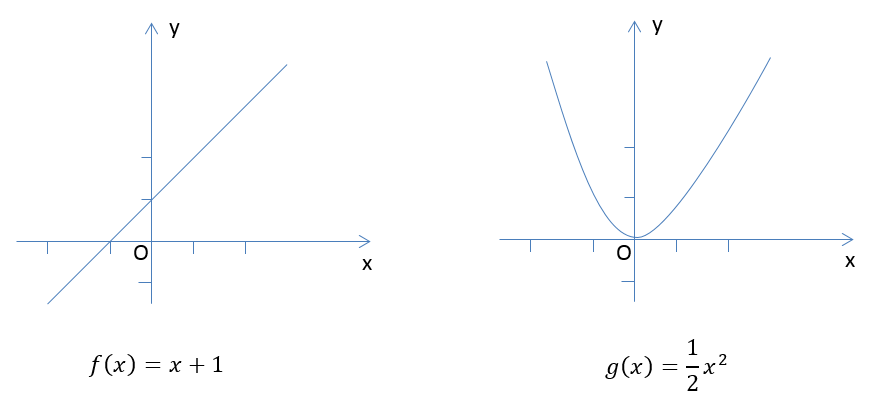
\includegraphics[scale=.6]{hinh9}

a) $f(-2)=1;f(-1)=0;f(0)=1;f(2)=3;g(-2)=\frac{1}{2};g(0)=0.$

b) $f(x)=2 \Leftrightarrow x+1=2 \Leftrightarrow x=1$.

Vậy với $x=1 thì f(x)=2$

$g(x)=2 \Leftrightarrow \frac{1}{2} x^2=2 \Leftrightarrow x^2=4 \Leftrightarrow x=2$ hoặc $x=-2.$ 

Vậy với $x=2$ hoặc $x=-2$ thì $g(x)=2$.

{\bf 4.Hàm số hợp}

\textit{Khái niệm hàm số hợp lớp 11}

Cho hai hàm số $y=f(u)và u=u(x).$ Thay thế biến u trong biểu thức $f(u)$ bởi biểu thức $u(x)$, ta được biểu thức $f[u(x)]$     với biến $x$. Khi đó, hàm số $y=g(x)$ với $g(x)=f[u(x)]$ được gọi là hàm số hợp của hai hàm số $f $và $u$; hàm số $u$     được gọi là hàm số trung gian.

{\bf Ví dụ}.Cho hai hàm số $y=f(u)$  và $u=u(x)$,trong đó

           $f(u)=u^2$  và $u(x)=x^2+3x+1.$
           
Nếu trong $f(u)$ ta thay thế biến $u$ bởi $u(x)$ thì được.
\begin{center}
$f[u(x) ]=(x^2+3x+1)^2$
\end{center}
\textit{Khái niệm hàm số hợp theo lí thuyết tập hợp.}

Giả sử $u=g(x)$ là hàm số của $x$, xác định trên $\left(a,b\right)$ lấy giá trị trên $\left(c,d\right)$, $y=f(u)$ là hàm số của $u$ xác định trên $\left(c,d\right)$ lấy giá trị trên $\mathbb{R}$. Khi đó ta lập một hàm số xác định trên $\left(a,b\right)$ lấy giá trị trên $\mathbb{R}$ theo quy tắc:

 \begin{center}
$x \longmapsto f\left[ {g(x)} \right]$
\end{center}
Ta gọi hàm $y=f[(g(x))]$ là hàm hợp của hàm số $y=f(u)$ và $u=u(x)$.\\
{\bf Ví dụ}. Cho ánh xạ
\begin{align*}
\text{ \space}f:\mathbb{R}&\longrightarrow\mathbb{R}\\
x&\longmapsto 2x-3
\end{align*}
\begin{align*}
\text{ \space}g:\mathbb{R}&\longrightarrow\mathbb{R}\\
x&\longmapsto \cos x-\sin x
\end{align*}
$f_{o}g=f\left[g(x)\right]=f\left(sinx\right)=2(\cos x-\sin x)-3=2cosx-2sinx-3$

\textit{Dựa vào định nghĩa hàm hợp ta thấy khái niệm hàm hợp chính là khái niệm thu hẹp của ánh xạ trong chương trình toán học cao cấp.}
\subsection{Ánh xạ và nội dung dạy học dãy số ở phổ thông}

{\bf 1. Định nghĩa}\\
{\bf Sách giáo khoa lớp 11 đã định nghĩa dãy số như sau}: Một hàm số $u$ xác định trên tập hợp các số nguyên dương $\mathbb{N^*}$ được gọi là một dãy số vô hạn (hay còn gọi tắt là dãy số).\\
Mỗi giá trị của hàm số $u$ được gọi là một số hạng của dãy số:\\
$u(1)$ được gọi là số hạng thứ nhất (hay số hạng đầu)\\
$u(2)$ được gọi là số hạng thứ hai\\
$... ... ...$\\
Người ta thường kí hiệu các giá trị $u(1), u(2),...$ tương ứng bởi $u_{1},u_{2},...$\\
{\bf Kí hiệu}
Người ta thường kí hiệu dãy số $u=u(n)$ bởi $(u_n)$, và gọi $u_n$ là số hạng tổng quát của dãy số đó.\\
Người ta cũng thường viết dãy số $u(n)$ dưới dạng khai triển:\\
\begin{center}
$u_1, u_2, ... , u_n, ...$
\end{center}
{\bf Ví dụ}\\
1.Hàm số $u_n=\frac{1}{n+1}$ xác định trên tập $\mathbb N^*$, là một dãy số. Dãy số này có vô số số hạng:\\
\begin{center}
$u_1=\frac{1}{2}, u_2=\frac{1}{3}, u_3=\frac{1}{4}, ...$
\end{center}
Khi viết dãy số dưới dạng khai triển ta được:\\
\begin{center}
$\frac{1}{2}, \frac{1}{3}, \frac{1}{4}, ..., \frac{1}{n+1}$
\end{center}
2. Dãy các số tự nhiên lẻ $1, 3, 5, 7, ...$ có số hạng đầu $u_1=1$, số hạng tổng quát $u_n=2n-1$.\\
{\bf Định nghĩa dãy số nhìn theo quan điểm ánh xạ}: \textit{Một dãy số là một ánh xạ từ $\mathbb{N}$ vào $K$ ($K=\mathbb{R}$ hoặc $\mathbb{C}$)}\\
{\bf Kí hiệu}
\begin{align*}
\text{ \space}u:\mathbb{N}&\longrightarrow\mathbb{K}\\
n&\longmapsto u(n)
\end{align*}
thay cho việc kí hiệu như trên , ta thường kí hiệu $(u_n)_{n \in \mathbb{N}}$ hay $(u_n)_{n \ge 0}$ hay $(u_n)$\\
{\bf Ví dụ}. Ánh xạ:
\begin{align*}
\text{ \space}u:\mathbb{N^*}&\longrightarrow\mathbb{K}\\
n&\longmapsto u(n)=n^2
\end{align*}
là một dãy số, khi viết dưới dạng khai triển ta được dãy các số chính phương:
\begin{center}
$1, 4, 9, 16, ...$, có số hạng đầu là $u_1=1$,số hạng tổng quát là $u_n=n^2$
\end{center}
\textit{Chú ý:} Mỗi ánh xạ từ$ \left\{n \in \mathbb N, n \ge n_o\right\}$ vào $K$, với $n_o \in K$ cố định cũng gọi là một dãy số.\\
{\bf 2.Cách cho một dãy số}\\
Người ta thường cho dãy số bằng một trong các cách sau đây:\\
{\bf Cách 1:} Dãy số cho bằng công thức của số hạng tổng quát\\
{\bf Ví dụ}. Cho dãy $(u_n)$ với $u_n=\frac{(-1)^{n+1}}{n^2}$. Nếu viết dãy số dưới dạng khai triển, ta được:
\begin{center}
$1, \frac{-1}{4}, \frac{1}{9}, ,..., \frac{(-1)^{n+1}}{n^2}, ...$
\end{center}
{\bf Cách 2}. Cho dãy số bằng phương pháp mô tả.\\
{\bf Ví dụ}: Cho dãy số $(u_n)$ với $u_n$ là giá trị gần đúng thiếu của số $ \pi$ với sai số tuyệt đối ${10}^{-n}$ .
Chẳng hạn, với $ \pi=3,1415926535...$
\begin{center}
Ta có $u_1=3,1 ; u_2=3,14 ; u_3=3,141 ; u_4=3,1415,... $
\end{center}
{\bf Cách 3}.Dãy số cho bằng phương pháp truy hồi\\
Tức là cho số hạng đầu (hay vài số hạng đầu) và cho hệ thức truy hồi tức là hệ thức biểu thị số hạng thứ $n$ qua số hạng (hay vài số hạng) đứng trước nó.\\
{\bf Ví dụ}. Cho dãy số 
$\left\{ \begin{array}{l}
u_1=2\\
u_n=u_{n-1}+3 (n \ge 2)                          
\end{array} \right.$\\
Ta có $u_1=2, u_2=2+3=5, u_3=5+3=8, u_4=8+3=11, ... $\\
{\bf3. Dãy số tăng, dãy số giảm và dãy số bị chặn}\\
- Dãy số $u_n$ được gọi là dãy số tăng (tăng ngặt) nếu ta có $u_{n+1} > u_n$ với mọi $n \in \mathbb{N}^*$\\
- Dãy số $u_n$ được gọi là dãy số giảm (giảm ngặt) nếu ta có $u_{n+1} < u_n$ với mọi $n \in \mathbb{N}^*$\\
- Các dãy số tăng, giảm được gọi chung là dãy đơn điệu.\\
- Các dãy số tăng ngặt, giảm ngặt được gọi chung là dãy đơn điệu ngặt.\\
\textit{Mỗi dãy đơn điệu đều là một đơn ánh.}\\
\textbf{Chú ý}: Không phải mọi dãy số đều tăng hoặc giảm. Chẳng hạn, dãy số $u_n$ với $u_n=(-3)^n$, tức là dãy\\
\begin{center}
$-3, 9, -27, 81, ...$
\end{center}
không tăng và cũng không giảm.\\
- Dãy số $(u_n)$ được gọi là bị chặn trên nếu tồn tại một số $M$ sao cho \\
\begin{center}
$u_n \le M, \forall n \in \mathbb{N}^*$
\end{center}
- Dãy số $(u_n)$ được gọi là bị chặn dưới nếu tồn tại một số $m$ sao cho \\
\begin{center}
$u_n \ge m, \forall n \in \mathbb{N}^*$
\end{center}
- Dãy số $(u_n)$ được gọi là bị chặn nếu nó vừa bị chặn trên vừa bị chặn dưới, tức là tồn tại các số $m, M$ sao cho\\
\begin{center}
$m \le u_n \le M, \forall n \in \mathbb{N}^*$
\end{center}
\textit{Chú ý}: Các dãy số hữu hạn luôn luôn bị chặn nên việc đưa ra định nghĩa trên chỉ thực sự ý nghĩa đối với các dãy vô hạn.\\
\textbf{4. Một số dãy số đặc biệt: Cấp số cộng, cấp số nhân}\\
\textbf{Cấp số cộng} là một dãy số (hữu hạn hoặc vô hạn), trong đó kể từ số hạng thứ hai, mỗi số hạng đều bằng số hạng đứng ngay trước nó cộng với một số không đổi $d$.\\
Do đó trong cấp số cộng ta có:\\
\begin{center}
$u_{n+1}=u_n+d$
\end{center}
{\bf Ví dụ}. Dãy số $1, -3, -7, -11, -15$ là một cấp số cộng với công sai $d=-4$\\
Đối với mỗi cấp số cộng $(u_n)$ ta luôn có các công thức sau:
\begin{center}
$u_n=u_1+(n-1)d , n \ge 2$\\
$u_k=\frac{u_{k-1}+u_{k+1}}{2} , k \ge 2$\\
$S_n=\frac{n(u_1+u_n)}{2}=nu_1+\frac{n(n-1)}2{d}$
\end{center}
\textit{Cơ sở của định nghĩa cấp số cộng là ánh xạ}:\\
\begin{align*}
\text{ \space}u:\mathbb{N^*}&\longrightarrow\mathbb{K}\\
n&\longmapsto u_{n+1}=u_n+d 
\end{align*}
\textbf{Cấp số nhân} là một dãy số ( hữu hạn hoặc vô hạn ),trong đó kể từ số hạng thứ hai, mỗi số hạng đều là tích của số hạng đứng ngay trước nó với một số không đổi $q$.Số $q$ dược gọi là công bội của cấp số nhân.\\
Do đó trong cấp số nhân ta có:\\
\begin{center}
$u_{n+1}=u_n.q$
\end{center}
{\bf Ví dụ}. Dãy số $-4, 1, \frac{-1}{4}, \frac{1}{16}, \frac{-1}{64}$ là một cấp số nhân với công bội $q=\frac{-1}{4}$\\
Đối với mỗi cấp số nhân $(u_n)$ ta luôn có các công thức sau:\\
\begin{center}
$u_n=u_1.q^{n-1} , n \ge 2$.\\
$u^{2}_{k}=u_{k-1}.u_{k+1} , k \ge 2$\\
$S_n=\frac{u_1(1-q^n)}{1-q}$
\end{center}
\textit{Cơ sở của định nghĩa cấp số nhân là ánh xạ}\\
\begin{align*}
\text{ \space}u:\mathbb{N^*}&\longrightarrow\mathbb{K}\\
n&\longmapsto u_{n+1}=u_n.q 
\end{align*}




\subsection{Ánh xạ và nội dung dạy học đại số tổ hợp ở phổ thông}
\textbf{1. Hoán vị}

{\bf a) Hoán vị có lặp}

{\bf Định nghĩa}: Có $n$ vật $(n \ge 1)$ được sắp xếp vào $n$ vị trí trong đó:\\
      có $n_1$  vật loại 1\\
      có $n_2$  vật loại 2\\
      $…   …   …$\\
      có $n_k$  vật loại $k$\\
ở đây $n_1+n_2+...+n_k$=$n$\\
mỗi cách sắp xếp thứ tự n vật như trên vào $n$ vị trí gọi là hoán vị có lặp của $n$ phần tử đó\\
{\bf Công thức tính}\\
Kí hiệu $C_n (n_1,n_2,…,n_k)$ là số các hoán vị của $n$ phần tử\\
\begin{center}
$C_{n}(n_1,n_2,...,n_k)=\frac{n! }{n_1!  n_2! ...n_k! }$
\end{center}
{\bf Ví dụ}
Có bao nhiêu chuỗi kí tự khác nhau bằng cách sắp xếp các chữ cái của từ $SUCCESS.$\\
{\bf Giải}
Trong từ SUCCESS có :\\ 
                                       3 chữ $S$\\
                                       1 chữ $U$.\\
                                       2 chữ $C$.\\
                                       1 chữ $E$.\\
Do đó số chuỗi có được là: $C_7= \frac{7!}{3!.1!.2!.1!}=420.$\\
{\bf b) Hoán vị vòng tròn}\\
{\bf Định nghĩa}:Cho tập $A$ gồm $n$ phần tử. Mỗi cách săp xếp $n$ phần tử này vào $n$ vị trí theo một đường tròn gọi là một hoán vị vòng tròn của tập hợp$A$ .Kí hiệu số hoán vị vòng tròn của$n$ phần tử là $P_(n-1)$.\\
{\bf Công thức tính}\\
\begin{center}
$P_(n-1)=(n-1)(n-2)…2.1=(n-1)!$
\end{center}
{\bf Ví dụ}.Có bao nhiêu cách xếp 5 sinh viên vào 1 vòng tròn?\\
{\bf Giải}\\
Đặt 1 sinh viên làm mốc, bài toán trở thành bài toán tính số hoán vị của 4 phần tử.\\
Do đó có tất cả $1.4!=24$ cách.\\
{\bf c) Hoán vị không lặp}\\
{\bf Định nghĩa}: Cho tập $A$ gồm $n$ phần tử. Mỗi cách sắp xếp $n$ phần tử này thành một dãy theo thứ tự xác định gọi là một hoán vị của tập hợp $A$.\\
{\bf Công thức tính}\\
Số các hoán vị của $n$ phần tử kí hiệu là $P_n$  được tính bằng công thức:\\
 \begin{center}
$P_n=n(n-1)…2.1=n!$
\end{center}

{\bf Ví dụ}: Xếp 3 người $a,b,c$ vào một cái bàn gồm 3 chỗ ngồi sẽ có $P_3=3!=6$ cách xếp đó là các cách sau: $$(a,b,c);(a,c,b);(b,a,c);(b,c,a);(c,a,b);(c,b,a)$$

{\bf Nhận xét}:\textit{ Theo quan điểm của ánh xạ thì: Số các hoán vị của tập hợp $n$ phần tử bằng số các đơn ánh (đồng thời cũng là song ánh) từ tập $n$ phần tử vào tập $n$ phần tử bằng $n!.$.}

\textit{Một song ánh từ tập $A$ lên tập $A$ còn được gọi là một phép thế vì vậy ta có thể có phát biểu như sau: Số các hoán vị của một tập hợp $n$ phần tử bằng số các phép thế của tập hợp đó và bằng $n!$.}

\textbf{2) Chỉnh hợp }

\textbf{a) Chỉnh hợp lặp.}

\textbf{Định nghĩa.}

Cho tập X gồm n phần tử $(n\in \mathbb{N}^*)$ một dãy có độ dài k $(k\in \mathbb{N}^*)$ các phần tử của $X$, trong đó mỗi phần tử có thể lặp lại nhiều lần, sắp xếp theo thứ tự nhất định gọi là một chỉnh hợp lặp chập k của $n$ phần tử. 

Kí hiệu số chỉnh hợp lặp chập k của n phần tử là: $F_n^k.$

Một số tài liệu kí hiệu số chỉnh hợp lặp chập k của n phần tử là: $\overline{A_n^k}$

\textit{Nhận xét: Theo quan điểm của ánh xạ thì: Mỗi chỉnh hợp chập k của n phần tử có thể xác định một ánh xạ từ tập $\{1,2,…,k\}$ đến tập n phần tử đó. Chẳng hạn chỉnh hợp lặp }

chập 5 (a,a,b,c,b) của 3 phần tử a,b,c xác định từ tập {1,2,3,4,5} đến 3 phần tử đó như sau: $\begin{pmatrix}
1 &2  &3  &4  &5 \\ 
 a&a  &b  &c  &b 
\end{pmatrix} $. 
Ngược lại mỗi ánh xạ từ tập $\{1,2,3,…,k\}$ đến tập $X$ xác định chỉnh hợp lặp chập 5 $(a,,a,b,c,b)$ của 3 phần tử $a,b,c.$

Như vậy tương ứng 1-1 giữa tập hợp ánh xạ từ tập $\{1,2,3,…,k\}$ đến tập $X$ và tập các chỉnh hợp lặp chập k của n phần tử của X. Điều đó có nghĩa là: Số chỉnh hợp lặp chập k của n phần tử của X bằng số các ánh xạ từ tập k phần tử đến tập n phần tử.


\textbf{Công thức tính.}
                    $$F_n^k=n^k$$
                    
Chứng minh.

Cho tập $X=\{x_1,x_2,…,x_n \}$, dãy có độ dài k là $\{a_1,a_2,…,a_k \}(k\in \mathbb{N}^*)$

     $a_1$ có n cách chọn.

     $a_2$ có n cách chọn ( vì  $a_2$ cũng có thể giống $a_1$ )

     $\cdots \cdots \cdots $

     $a_k$ cũng có n cách chọn.
     
Vậy dãy có độ dài k có $n^k$ cách chọn hay $F_n^k=n^k.$

Ví dụ.

1) Có bao nhiêu số tự nhiên có 4 chữ số được viết từ các số tự nhiên lẻ.

2) Biển đăng kí oto có 6 chữ số và hai chữ cái đầu tiên trong 26 chữ cái (không dùng $O$ và $I$). Hỏi số ô tô được đăng kí nhiều nhất là bao nhiêu?

Giải.

a) Gọi X là tập hợp các số tự nhiên lẻ có một chữ số thế thì $X=\{1,3,5,7,9\}$ như vậy tập X gồm 5 phần tử. 

Do đó các số tự nhiên lẻ có 4 chữ số được tạo ra từ tập X là: $F_5^4=5^4=625$ số.

b) Gọi X là tập hợp các chữ cái dùng trong biển đăng kí suy ra X có 24 phần tử vì không dùng chữ O và chữ I. Chọn 2 chữ cái trong 24 chữ có $F_24^2=24^2$ cách chọn. Gọi Y là tập hợp các số dùng trong bảng đăng kí, suy ra Y có 10 phần tử $(Y=\{0,1,2,3,4,5,6,7,8,9\})$. Chọn 6 số trong tổng số 10 có $F_10^6=10^6$ cách chọn. Do đó có tất cả $24^2.10^6$ biển số được tạo ra.

\textbf{b) chỉnh hợp không lặp.}

Định nghĩa.

Cho tập A gồm m phần tử $x_1,x_2,..,x_m$ và số nguyên dương n với $1\le n\le m$. Ta thiết lập bộ $ (a_1,a_2, \cdots ,a_n ) | a_i \in A \forall i=\overline{1,n},a_i$ khác nhau từng đôi một được gọi là  một chỉnh hợp không lặp chập n của m phần tử đã cho. Số các chỉnh hợp không lặp chập n của m phần tử kí hiệu là: $A_m^n$

Nhận xét:
Theo quan điểm ánh xạ. Mỗi chỉnh hợp chập n của m phần tử đã cho có thể xác định một đơn ánh từ tập $\{1,2,...,n\}$ đến tập m phần tử đó. Chẳng hạn, chỉnh hợp chập 2 $(a,c)$ của 3 phần tử a,b,c xác định đơn ánh từ tập $\{1,2\}$  đến tập chứa 3 phần tử a,b,c như sau: $$\begin{pmatrix}
1 &2 \\ 
 a&c 
\end{pmatrix}$$

Ngược lại, mỗi đơn ánh từ tập $\{1,2,..,n\}$ đến tập m phần tử đó xác định một chỉnh hợp chập n của m phần tử. Chẳng hạn đơn ánh  $ \begin{pmatrix}
1 &2 \\ 
 a&c 
\end{pmatrix}$ xác định chỉnh hợp chập 2 của 3 phần tử $a,b,c.$

Như vậy có tương ứng 1-1 giữa tập hợp các đơn ánh từ tập $\{1,2,…,n\}$ đến tập m phần tử của $A( n\le m)$ và tập các chỉnh hợp chập n của m. Điều đó có nghĩa là: số chỉnh hợp chập n của m phần tử của tập hợp $A(n\le m)$ bằng số các đơn ánh từ tập n phần tử vào tập m phần tử.


• Công thức tính.
$$A_m^n=m(m-1)…(m-n+1)= \frac{m!}{(m-n)!}$$

Chứng minh( theo quan điểm ánh xạ)

Ta kí hiệu số các đơn ánh từ $\{1,2,…,n\}$ đến tập A gồm m phần tử là $A_m^n$

Chẳng hạn:    

$A_m^1$  là số đơn ánh từ $\{1\}$  đến tập A.
$A_m^2$  là số đơn ánh từ $\{1,2\}$  đến tập A.

$\cdots \cdots \cdots $

Rõ ràng ta có $A_m^1=m$

Để tìm công thức cho $A_m^n$  ta tìm  mối liên hệ giữa $A_m^{n-1}$  và $A_m^n$  .Ta nhận thấy mỗi đơn ánh từ tập $\{1,2,…,n-1\}$ đến tập A có $m-(n-1)$ cách mở rộng thành đơn ánh từ tập $\{1,2,…,n-1,n\}$ đến tập A bằng cách cho tương ứng n lần lượt với $m-(n-1)$  phần tử còn lại không phải ảnh của $1,2,...,n-1.$

Như vậy ta có: $A_m^n=[m-(n-1)] A_m^{n-1}=(m-n+1) A_m^n$

Lần lượt áp dụng công thức trên ta có:
\begin{align*}
A_m^2 &= (m-2+1) A_m^1=(m-1)m\\ 
 A_m^3&=(m-3+2) A_m^2=(m-2)(m-1)m \\ 
A_m^4 &= (m-4+1)A_m^3=(m-3)(m-2)(m-1)m\\
&\cdots \cdots \cdots 
\end{align*}

Cuối cùng ta được: $A_m^n=m(m-1)…(m-n+1)=\frac{m!}{(m-n)!}$

Chú ý: Một chỉnh hợp chập m của m phần tử được gọi là một hoán vị của m phần tử.
    $$ A_m^m=P_m=m!$$

\textbf{Ví dụ.}

	 Có bao nhiêu số tự nhiên có 4 chữ số đôi một khác nhau được viết từ những số tự nhiên lẻ.
	 
	Với các số $\{0,1,2,3,4,5\}$
	
        +) Có thể lập được bao nhiêu số tự nhiên lẻ gồm 4 chữ số khác nhau.
        
        +) Có thể lập được bao nhiêu số tự nhiên chẵn gồm 4 chữ số khác nhau.
        
\textbf{Giải.}

1) Gọi X là tập hợp các số tự nhiên lẻ có một chữ số, $X=\{1,3,5,7,9\}$ suy ra X có 5 phần tử. Chọn 4 số đôi một khác nhau trong tập X gồm 5 phần tử chính là chỉnh hợp không lặp chập 4 của 5. Do đó số các số tự nhiên có 4 chữ số đôi một khác nhau được viết từ các số lẻ là: $A_5^4=5.4.3.2.1=120$ số .

2) +) gọi số cần tìm có dạng: $\overline{a_1a_2a_3a_4} $

 $a_4  \in \{1,3,5\}$  do đó $a_4$  có 3 cách chọn

$ a_1\neq 0$ nên có 4 cách chọn.

2 chữ số còn lại có $A_2^4$  cách chọn.

Vậy có tất cả là $4.3.A_2^4=144$ số.

+) gọi số cần tìm có dạng: $\overline{a_1a_2a_3a_4}$

TH1: $a_4=0$ nên có 1 cách chọn

         Chọn 3 số còn lại trong 5 số có $A_3^5$  cách chọn

         Do đó có $1.A_3^5$  số.

TH2: $a_4\neq 0$ nên có 2 cách chọn.

          $a_1$  có 4 cách chọn.

Chọn 2 số còn lại trong 4 số có $A_2^4$  cách chọn.

Do đó có $1.A_3^5$  số

Vậy  có tất cả $1.A_3^5+1.A_3^5=156$ số thỏa mãn yêu cầu bài toán.


\subsection{Các phép toán nhìn theo quan điểm ánh xạ.}
    Dùng khái niệm ánh xạ người ta đã định nghĩa phép toán đại số trên một tập hợp cho trước. Khi các tập hợp đã cho là các tập số ta có những phép toán trên các tập hợp số.\\
    Một số phép toán đại số hai ngôi được xét trong chương trình môn Toán ở phổ thông cùng những tính chất và các phần tử đặc biệt.\\


\begin{tabular}{|p{1.8cm}|c|p{2cm}|p{3cm}|p{3cm}|p{3cm}|}
\hline 
 &  & \multicolumn{2}{c|}{Loại phép toán} &  &  \\ 
\hline 
 &  & Toàn cục hay bộ phận & Điều kiện &  &  \\ 
\hline 
Cộng trên $\mathbb{N}$ & + & Toàn cục &  & Giao hoán, kết hợp, luật giản ước & Trung hòa 0, lũy đẳng 0 \\ 
\hline 
Nhân trên $\mathbb{N}$ & . & Toàn cục &  & Giao hoán, kết hợp, phân phối với phép toán + và - &Đơn vị 1; lũy đẳng 1;0. Phần tử giản ước được $a\neq 0$   \\ 
\hline 
Trừ trên $\mathbb{N}$ & - & Bộ phận & a-b với $a\ge b$ &  &Đơn vị phải 0, lũy đẳng 0 \\ 
\hline 
Chia trên $\mathbb{N}$& : & Bộ phận & A chia hết cho B $\Leftrightarrow \exists c \in \mathbb{N} (a=bc)$ &  & Đơn vị phải 1, lũy đẳng 1 \\ 
\hline 
Cộng trên $\mathbb{Z}$& +& Toàn cục &  & Giao hoán, kết hợp, $\forall a\in \mathbb{Z},\exists (-a) \in \mathbb{Z}$ & Trung hòa 0, lũy đẳng 0  \\ 
\hline 
Nhân trên $\mathbb{Z}$ & . & Toàn cục &  & Giao hoán, kết hợp, phân phối với phép  toán+ và - & Đơn vị 1, lũy đẳng 1;0 \\ 
\hline 
\end{tabular} 






\subsection{Một số loại ánh xạ khác trong chương trình Toán phổ thông}
\textbf{a) Hàm mệnh đề}\\
    Ánh xạ từ tập $D$ vào tập $I=\left\{0,1\right\}$ được gọi là vị từ ( hay hàm mệnh đề) trên tập $D$.\\
    Trong môn Toán ở phổ thông khái niệm hàm mệnh đề đứa gọi là mệnh đề chứa biến. Khái niệm này được sử dụng để định nghĩa phương trình và bất phương trình.\\
{\bf Ví dụ}\\
1. Khái niệm phương trình một ẩn.\\
" Phương trình ẩn $x$ là mệnh đề chứa biển có dạng\\
\begin{center}
$f(x)=g(x)  ,         (1)$
\end{center}
trong đó $f(x)$ và $g(x)$ là những biểu thức của $x$. Ta gọi $f(x)$ là vế trái, $g(x)$ là vế phải của phương trình (1) .\\
Nếu có số thực $x_o$ sao cho $f(x_o)=g(x_o)$ là mệnh đề đúng thì $x_o$ được gọi là một nghiệp của phương trình (1). Giải phương trình (1) là tìm tất cả các tập nghiệm của nó. Nếu phương trình không có nghiệm nào thì ta nói phương trình vô nghiệm (hoặc nói tập nghiệm của nó là rỗng)"\\
2. Khái niệm bất phương trình một ẩn.\\
"Bất phương trình ẩn $x$ là mệnh đề chứa biến có dạng\\
\begin{center}
$f(x)<g(x)         , (f(x) \ge g(x))$,          (1)
\end{center}
trong đó $f(x)$ và $g(x)$ là những biểu thức của $x$.\\
Ta gọi $f(x)$ và $g(x)$ lần lượt là vế trái và vế phải của bất phương trình (1). Số thực $x_o$ sao cho $f(x_o)<g(x_o) (f(x_o) \ge g(x_o))$ là mệnh đề đúng được gọi là một nghiệm của bất phương trình (1).giải bất phương trình là tìm tập nghiệm của nó, khi tập nghiệm rỗng thì ta nói bất phương trình vô nghiệm."\\
\textbf{b) Đạo hàm của hàm số}\\
Mỗi hàm số $f(x)$ xác định và có đạo hàm trên khoảng $(a,b)$ xác định một hàm số $f^{'}(x)$ trên khoảng $(a,b)$. \textit{Tương ứng $f(x)$ với $f^{'}(x)$ cho ta một ánh xạ biến $f(x)$ thành $f^{'}(x)$}. Ánh xạ này có tính cộng tính và thuần nhất, tức là:\\
\begin{center}
$(f(x)+g(x))^{'}=f^{'}(x)+g^{'}(x)$\\
$(kf(x))^{'}=kf^{'}(x)$, $k$ là hằng số.
\end{center}
\textbf{c) Tích phân của hàm số}\\
Mỗi hàm số $f(x)$ khả tích trên $\left[a,b\right]$xác định một số $\int\limits_a^b {f(x)dx}$ .\textit{Tương ứng $f(x)$ với $\int\limits_a^b {f(x)dx}$ là một ánh xạ từ tập hợp các hàm khả tích trên $\left[a,b\right]$ đến tập hợp số thực $\mathbb{R}$}. Ánh xạ này có tính chất cộng tính và thuần tính. Tức là:\\

$$\int\limits_a^b {(f(x) + g(x))dx}  = \int\limits_a^b {f(x)dx}  + \int\limits_a^b {g(x)dx} $$
$$\int\limits_a^b {(kf(x))dx = k\int\limits_a^b {f(x)dx} } $$


\subsection{Ánh xạ với nội dung dạy học phép biến hình ở phổ thông.}
 \medskip
 
   
       Dạy học phép biến hình ở phổ thông  có mối liên hệ mật thiết với khái niệm ánh xạ trong toán học cao cấp. Các phép biến hình có thể được xem như những ánh xạ giữa các tập hợp điểm trong mặt phẳng hay trong không gian.\\
\medskip
       Khi xét các phép biến hình trong mặt phẳng hay trong không gian theo quan điểm ánh xạ ta thường xét đến các bất biến, tích (hợp thành) của các phép biến hình và lợi dụng các bất biến đẻ giải một số dạng toán và giải quyết các tình huống thực tiễn.
\medskip  \\
       Phép đo các đại lượng hình học ( độ dài, diện tích, thể tích) có thể xét như lừ các ánh xạ cho ứng mỗi hình nào đó với một số thực không âm xác định thông qua một đơn vị cho trước. Không phải hình nào cũng có số đo được xác định. Ánh xạ trong phép đo các đại lượng hình học cần thỏa mãn những điều kiện nhất định.
       
-	Kiến thức về biến hình trong môn toán trung học cơ sở.


\begin{tabularx}{\textwidth}{|c|>{\raggedright}X|}
\hline
\textbf{Kiến thức } & \textbf{Nội dung} \tabularnewline
\hline
Đối xứng trục  & Hai điểm đối xứng qua một đường thẳng,   \\
   Hai hình đối xứng qua một đường thẳng; \tabularnewline
\hline
   Đối xứng tâm & Hai điểm đối xưng qua một điểm; Hai hình đối xứng qua một đường thẳng; Hình có trục đối xứng   \tabularnewline 
   \hline
   Tam giác đồng dạng& Khái niệm hai tam giác đồng dạng; Ba trường hợp đồng dạng của tam giác;    Các trường hợp đồng dạng của tam giác vuông;
   ứng dụng thực tế của tam giác đồng dạng\tabularnewline

\hline
\end{tabularx}

-	Kiến thức về phép biến hình trong môn toán trung học phổ thông.


\begin{tabular}{|p{4.5cm}|p{9cm}|}
\hline
\textbf{Kiến thức } & \textbf{Nội dung} \tabularnewline
\hline
Khái niệm phép biến hình  &  \tabularnewline
\hline
  Phép tịnh tiến & Định nghĩa phép tịnh tiến trong mặt phẳng; Các tính chất của phép tịnh tiến trong mặt phẳng; Biểu thức tọa độ của phép tịnh tiến.   \tabularnewline 
   \hline
Phép đối xứng trục& Định nghĩa phép đối xứng trục; Biểu thức tọa độ của phép đối xứng trục; Các tính chất của phép đối xứng trục; Trục đối xứng của một hình. \tabularnewline

\hline
Phép đối xứng tâm&Định nghĩa phép đối xứng tâm; Biểu thức tọa độ của phép đối xưng tâm; Các tính chất của phép đối xưng tâm; Tâm đối xứng của một hình. \tabularnewline
\hline
Phép quay&Định nghĩa phép quay; Các tính chất của phép quay \tabularnewline 
\hline
Khái niệm phép dời hình và hai hình bằng nhau&Khái niệm phép dời hình; Tính chất của phép dời hình; Định nghĩa hai hình bằng nhau qua phép dời hình. \tabularnewline
\hline 
Phép vị tự&Định nghĩa phép vị tự; Tính chất của phép vị tự; Tâm vị tự của hai đường tròn. \tabularnewline
\hline
Phép đồng dạng.&Định nghĩa phép đồng dạng; Tính chất của phép đồng dạng; Hình đồng dạng. \tabularnewline
\hline
Phép chiếu song song& \tabularnewline
\hline
\end{tabular}

Sau đây chúng ta sẽ đi xét một số ví dụ để thấy được mối liên hệ của ánh xạ với nội dung dạy học phép biến hình.

\textbf{1. Phép biến hình}
\textbf{a) Định nghĩa.}

Phép biến hình( trong mặt phẳng) là một quy tắc để mỗi điểm $M$ thuộc mặt phẳng xác định được duy nhất một điểm $M’$ thuộc mặt phẳng ấy.

\textbf{Nhận xét:} đối chiếu với khái niệm ánh xạ ta thấy rằng phép biến hình thực chất là một ánh xạ.Do đó theo theo quan điểm ánh xạ định nghĩa trên được phát biểu như sau: 

(H) là một hình tùy ý trong mặt phẳng, $F$ là một phép biến hình trong mặt phẳng thế thì: 

\centerline {\fullfunction{F}{(H)}{(H')=F(H)}{\forall M\in (H)}{F(M)=M'\in(H')}}

Phép biến hình  $F$ biến $(H)$ thành $(H') \Leftrightarrow (H') '=\{M'=F(M)|\forall M\in F(M)\}$

\textbf{b) Các ví dụ.}

\textbf{ví dụ 1:} Cho vecto $\overrightarrow{u}$. Với mỗi điểm M, ta xác định điểm M’ theo quy tắc $\overrightarrow{MM'} =\overrightarrow{u}$
quy tắc trên là một phép biến hình và được gọi là phép tinh tiến theo vecto $\overrightarrow{u}$.

\textbf{Ví dụ 2:} Xét quy tăc: Với mỗi điểm M, ta xác định điềm M’ trùng M. Quy tắc trên là một phép biến hình và được gọi là phép đồng nhất.

\textbf{Ví dụ 3.}Cho đường thẳng d. Với mỗi điểm $M\in d$ ta xác định điểm M’ là hình chiếu của  điểm M lên d. Quy tắc trên là một phép biến hình và được gọi là phép chiếu (vuông góc )lên đường thẳng d.

\textbf{Ví dụ 4.} Xét quy tắc: Cho điểm M cố định với mỗi điểm M ta xác định điểm M’ thỏa mãn $\overrightarrow{OM'}=\overrightarrow{OM}$. Quy tắc trên không là phép biến hình.

\textbf{2. Phép tịnh tiến.}

    \textbf{Định nghĩa }theo sách giáo khoa: Phép tịnh tiến theo vecto $\overrightarrow{u}$ là một phép biến hình  mỗi điểm M thành M’ sao cho $\overrightarrow{MM'}=\overrightarrow{u}.$

Phép tịnh tiến theo vecto $\overrightarrow{u}$ thường được kí hiệu là T hoặc $T_{\overrightarrow{u}}$ . Véctơ $\overrightarrow{u}$  được gọi là vecto tịnh tiến.

\textbf{Theo quan điểm ánh xạ }định nghĩa trên được phát biểu như sau:

"phép tịnh tiến theo vecto  biến điểm M thành M’ kí hiệu:

$T_{\overrightarrow{u}}:M \mapsto M'$ hay $T_{\overrightarrow{u}}=M'$

Khi đó $T_{\overrightarrow{u}}(M)=M' \Leftrightarrow \overrightarrow{MM'}=\overrightarrow{u}.$


Ví dụ. trong mặt phẳng oxy cho 2 điểm $A(1,-2), B(3,1)$ và $\overrightarrow{v}(1,0)$ Tìm tọa độ của 2 điểm $A’$ và $B$’ lần lượt là ảnh của A,B qua phép tịnh tiến theo $\overrightarrow{v}$   

$T_{\overrightarrow{v}}(A)=A'(2,-2),T_{\overrightarrow{v}}(B)=B'(4,1)$

\textbf{3. Phép đối xứng trục.}

   \textbf{   Định nghĩa:} cho đường thẳng d. Phép biến hình biến mỗi điểm M thuộc d thành chính nó, biến mỗi điểm $M$ không thuộc d thành $M’$ sao cho d là đường trung trực của đoạn $MM’$ được gọi là phép đối xứng qua đường thẳng d hay phép đối xứng trục d.
   
Đường thẳng d được gọi là trục của phép đối xứng hoặc đơn giản là trục đối xứng.

 Phép đối xứng trục d Kí hiệu là: $\text{Đ}_d $
Theo quan điểm ánh xạ :

" phép đối xứng trục $\text{Đ}_d$  biến M thành $M’$ được viết là:

$\text{Đ}_d:M\mapsto M' $ hay $\text{Đ}_d(M)=M'$

Khi đó $\text{Đ}_d:M\mapsto M' \Leftrightarrow M$ và $M'$ đối xứng với nhau qua $d$.

Phép đối xứng trục $\text{Đ}_d$ biến những điểm nằm trên đường thẳng thành chính nó:

$\text{Đ}_d:M\mapsto M' $ thì $\text{Đ}_d:M'\mapsto M$

$\text{Đ}_d:(H)\mapsto (H') $ thì $\text{Đ}_d:(H')\mapsto (H)$

\textbf{Ví dụ.} Cho điểm A và B nằm về một phía với đường thẳng d. Hãy xác định điểm M trên d sao cho tổng $AM+MB$ đạt giá trị nhỏ nhất.

Nếu hai điểm A,B nằm về hai phía của đường thẳng d thì điểm M cần tìm là giao của đoạn thẳng $AB$ và đường thẳng d.

Xét bài toán,  lấy điểm A’ đối xứng với A qua d. Khi đó :
                    $$AM+MB=A'M+MB$$

 $AM+MB$ nhỏ nhất khi $A,M,B$ thẳng hàng, $M=M_0=A'B \cap d$.

\textbf{4.Phép quay.}

\textbf{Định nghĩa: }Trong mặt phẳng cho điểm O và góc lượng giác $\varphi$ không đổi.  phép biến hình biến điểm O thành điểm O, biến mỗi điểm M (khác 0) thành điểm $M’$ sao cho $OM=OM’$ và $(OM,OM’)=\varphi$ được gọi là phép quay tâm O góc $\varphi$.

Kí hiệu: $Q_{(o,\phi)}$ , hoặc $\mathbb{Q}$ (trong trường hợp không cần chỉ rõ tâm và góc quay)
$\mathbb{Q}_{(o,\varphi)}:M\mapsto M'$  hay $\mathbb{Q}_{(o,\varphi)}(M)=M'$

Khi đó: $\mathbb{Q}_{(o,\varphi)}: M\mapsto M' \Leftrightarrow \left\{\begin{matrix}
OM=OM'\\ 
(OM,OM')=\varphi
\end{matrix}\right.$

Như vậy một phép quay hoàn toàn được xác định khi biết tâm quay và góc quay $\varphi$

\textbf{Ví dụ:} Trên một chiếc đồng hồ từ lúc $12$ giờ đến $15$ giờ kim giờ và kim phút đã quay một góc bằng $90^0$. Đó là một phép quay với tâm O là lúc kim phút  ở vị trí $12$ giờ và góc quay $\varphi=90^0$.


\newpage
\vspace*{0.2cm}
\centerline{\Large\bf KẾT LUẬN}
\medskip
Việc nghiên cứu: Ánh xạ và nội dung dạy học ánh xạ ở phổ thông giúp chúng ta liên kết những nội dung đã học ở Đại học với chương trình phổ thông. Góp phần nâng cao năng lực phân tích sách giáo khoa toán liên quan đến toán học cao cấp, toán học hiện đại, phát huy tính tích cực, chủ động của giáo viên trong quá trình dạy học.

\medskip
Do thời gian nghiên cứu không nhiều nên khóa luận chỉ nghiên cứu được một số nội dung toán ở phổ thông liên quan đến ánh xạ như: toán tiểu học, hàm số, dãy số,..và sẽ còn nhiều mối liên hệ nữa chưa đề cập đến trong khóa luận . Hi vọng các bạn sinh viên yêu thích môn đại số sẽ tiếp tục quan tâm đến vấn đề này.

\medskip
Mặc dù bản thân đã ra sức cố gắng, xong do hạn chế về trình độ chuyên môn nên khóa luận không tránh khỏi những sai xót. Rất mong nhận được sự đóng góp của quý thầy cô và các bạn sinh viên.
%%% vẽ hình chèn 1 file tex nằm trong cùng thư mục chứa khóa luận%%%
%\begin{figure}[h]
%	\verbatiminput{vd1.tex}
%	\caption{Kết quả tính toán cho Ví dụ 3.1.1 }\label{fig1}
%\end{figure}
\newpage

%\begin{figure}[h]
%	\centering
%	\includegraphics[scale=0.9]{D:/anhmatlab/vd2a.jpg}
%	\caption{Kết quả tính toán cho Ví dụ 3.1.2 với $x_{0}=3$ }\label{fig2a}
%\end{figure}

%\addcontentsline{toc}{chapter}{Tài liệu tham khảo}

% \begin{thebibliography}{99}
 
% \bibitem{CGT00}   {\sc A. R. Conn, N. I. M. Gould, and P. L. Toint}, {\it %Trust-Region Methods}, MPS-SIAM Series on Optimization, Philadelphia, %2000.
 
  
% \end{thebibliography}
 \end{document}
